% Preamble
\documentclass[12pt,twoside,openany]{book}

% Packages
\usepackage[utf8]{inputenc}
\usepackage[spanish]{babel}
\usepackage[T1]{fontenc}
\usepackage[width=150mm,top=25mm,bottom=25mm]{geometry}
\usepackage{caption}
\usepackage{subcaption}
\usepackage{pdfpages}
\usepackage{amsmath}
\usepackage[algoruled,noline,linesnumbered,spanish]{algorithm2e}
\usepackage[fixlanguage]{babelbib}

\usepackage[backref=page]{hyperref}
\backrefspanish
\renewcommand{\backref}[1]{}
\renewcommand{\backrefalt}[4]{%
\ifcase #1 \relax%
\or (Citado en la página~#2).%
\else (Citado en las páginas~#2).%
\fi%
}

\usepackage{graphicx}
\graphicspath{ {images/} }

\usepackage{fancyhdr}
\pagestyle{fancy}
\fancyfoot{}
\fancyhead{}
\renewcommand{\chaptermark}[1]{\markboth{\small \ \chaptername\ \thechapter. \ #1}{}}
\renewcommand{\sectionmark}[1]{\markright{\thesection \ \ #1}}
\fancyhead[L]{\slshape \leftmark}
\fancyhead[R]{\thepage}
\fancyhead[LO]{\slshape \rightmark}
\fancyhead[RO,LE]{\textbf{\thepage}}
\fancyhead[RE]{\slshape \leftmark}

\renewcommand{\frontmatter}{%
\pagenumbering{roman}
\pagestyle{plain}
}

\renewcommand{\mainmatter}{%
\cleardoublepage%
\pagenumbering{arabic}
\pagestyle{fancy}
}

\renewcommand{\backmatter}{%
\pagestyle{plain}
}


% Document
\begin{document}
    \frontmatter

    %    \includepdf{../out/title.pdf}

    %    \thispagestyle{plain}
\begin{center}
    \Large
    \textbf{Thesis Title}

    \vspace{0.4cm}
    \large
    Thesis Subtitle

    \vspace{0.4cm}
    \textbf{Eddy Nelson Almuiña Hernández}

    \vspace{0.9cm}
    \textbf{Abstract}
\end{center}
Lorem ipsum dolor\ldots

    \begin{flushright}
        \thispagestyle{empty}
        \emph{Hello, World!}
    \end{flushright}

    %    \chapter*{Acknowledgements}\label{ch:acknowledgements}
    %    I want to thank\ldots

    %    \tableofcontents
    %    \listoffigures
    %    \listoftables
    %    \listofalgorithms

    \chapter*{Introducción}\label{ch:introduction}
    %TODO Te falta el objeto de estudio que son los algoritmos de clasificación y los campos de acción es donde lo aplica en la detección de sonido

Desde su origen, el ser humano se ha visto interesado por el medio que le rodea.
Una parte de este medio a la que le ha prestado especial atención son los seres vivos que lo habitan, en especial los animales, con los que guarda mayor parentesco.
Su estudio le ha permitido comprender el modo en que funciona la naturaleza, y puesto que es parte de esta, el modo en que funciona su propio organismo.

La Biología no ha permanecido ajena a lo que ocurre con el resto de las ramas de la ciencia, se ha divido en áreas dedicadas a subcampos específicos, que mutan con el tiempo cual especies vivientes y que, en ocasiones se cruzan con otras ramas para dar origen a nuevos campos de estudio.
El anterior es el caso de la Bioacústica, hija de la Biología y la Acústica, dedicada a la comprensión de señales sonoras de origen biológico.

Durante años la Bioacústica vio su labor dificultada por problemas de índole tecnológica, el desarrollo científico estuvo lastrado por el de los medios necesarios para procesar la información disponible.
Esto ha cambiado recientemente con la introducción de dispositivos de grabación y almacenamiento de mayor calidad y capacidad y, especialmente, con la aplicación de técnicas de Inteligencia Artificial.

Un factor que afectó el avance científico en esta área era que las señales debían ser procesadas por expertos en la materia, quienes tenían la engorrosa tarea de segmentar\footnote{Segmentar es el procedimiento de separar una grabación sonora en porciones (segmentos) en las que ocurren una o varias señales acústicas de interés.} y clasificar cada grabación con el propósito de determinar la ocurrencia de sonidos emitidos por ciertas especies de animales en estas.
Los especialistas debían dedicar horas a este tedioso procedimiento, haciendo poco factible el desarrollo de estudios que requirieran la detección de especies mediante tal proceder.
Dichos estudios son muy necesarios para el desarrollo de proyectos ecológicos, medioambientales y de investigación de nuevas especies, sobre todo en lugares donde las condiciones geográficas y del entorno dificultan la observación directa.

La Inteligencia Artificial ha sido vista como una posible solución a la problemática antes planteada.
Son numerosos los estudios llevados a cabo con diferentes algoritmos de esta para su aplicación en la detección y clasificación de señales bioacústicas~\cite{Gerhard03}.
En general estos pueden ser clasificados en supervisados o no supervisados, de acuerdo a si requieren un conjunto de datos previamente procesados a partir de los cuales <<deducir>> el resultado para nuevos datos o no, respectivamente.
Algoritmos supervisados han sido ampliamente aplicados para la solución del problema en cuestión, quedando la pertinencia y calidad del uso de los no supervisados como un objeto de estudio menos abordado.

Entre las técnicas más estudiadas para la clasificación de señales bioacústicas encontramos:
\begin{itemize}
    \item Neural Networks~\cite{Gerhard03,Deecke05}
    \item K-Nearest Neighbours~\cite{Dunkel06}
    \item Support Vector Machines~\cite{Ilyas14}
    \item Decision Trees~\cite{Lasseck14}
    \item Naive-Bayes~\cite{Dunkel06}
\end{itemize}

Todas las técnicas antes mencionadas pertenecen al campo del aprendizaje supervisado por lo que, para su aplicación, están sujetas a la existencia de un conjunto de entrenamiento previamente etiquetado por expertos.

Son múltiples los problemas que debe enfrentar un sistema automatizado para la clasificación de una señal bioacústica: el ruido de fondo producido por especies emitiendo sonidos de forma simultánea;
el que producen eventos meteorológicos como la lluvia o el viento;
o las variaciones en la frecuencia de la señal que emite un individuo en dos momentos distintos, o diferentes individuos de una misma especie.
Todas constituyen dificultades a tratar cuando se desarrolla un mecanismo para responder a la interrogante de qué especie animal se escucha en un segmento de una grabación dada.

Una tendencia en numerosos trabajos es enfocarse en la clasificación de una categoría taxonómica específica como aves~\cite{Lasseck14,Oliveira15,Stowell14} o primates~\cite{Heinicke15}.
Lo anterior persigue lograr un mejor ajuste en los parámetros de los algoritmos y alcanzar así resultados de mayor calidad.
Se encuentra menos estudiada la aplicación en grabaciones sobre una comunidad de organismos diversa, donde los resultados han sido menos alentadores~\cite{Ilyas14}; y resulta un campo particularmente propicio para la aplicación de algoritmos no supervisados, dada su naturaleza de no requerir conocimiento previo de las categorías esperadas, y que funcionan mejor para mayores separaciones entre las categorías.

Planteado el contexto sobre el que se desarrolla este trabajo, formulamos la siguiente pregunta científica: ¿En qué escenarios resulta propicia la aplicación de algoritmos de aprendizaje no supervisado para la clasificación automática de señales sonoras?

Para dar respuesta a esta interrogante, nos proponemos cumplir los siguientes objetivos:
\begin{itemize}
    \item Presentar un estudio de los algoritmos de aprendizaje no supervisado y clustering semi-supervisado\footnote{Técnica que aplica algoritmos de aprendizaje no supervisado a conjuntos de datos en los que se conoce la categoría de algunos elementos.} y su aplicación en el procesamiento de señales.
    \item Implementar variantes de los algoritmos estudiados.
    \item Establecer una comparación entre los resultados obtenidos, en correspondencia con el problema general (clasificación de señales de diversas especies) y restricciones de este (clasificación de señales en categorías de especies específicas).
\end{itemize}

    \mainmatter

    \chapter{Extracción de Características}\label{ch:features}
    Una señal de sonido no es más que la variación en la presión que ejerce el medio que la transmite sobre su receptor.
La percepción del sonido en los seres humanos ocurre en dos regiones fundamentales: la \textit{periférica} y la \textit{nerviosa}.
Comienza en los oídos y continúa a través de la cóclea, en el oído interno, donde las variaciones en la presión del aire son transformadas en impulsos nerviosos conducidos hacia la corteza cerebral.

El hertz (Hz) es la unidad que expresa la cantidad de vibraciones que emite una fuente sonora en cada segundo de tiempo (frecuencia).
Se considera que el oído humano puede percibir ondas sonoras de frecuencias entre los 20 y los 20~000 Hz.
Los tonos agudos son percibidos en las frecuencias más altas (por encima de 5 kHz), y los graves en las bajas (menos de 250 Hz).

Un sonido puede ser representado de forma simple mediante un \textbf{oscilograma} (figura~\ref{img:oscillogram}), donde el eje X representa el tiempo, y el eje Y representa la \textit{amplitud} de la presión del sonido (generalmente usando unidades de media arbitrarias).
Mediante su análisis se pueden detectar con facilidad los instantes de tiempo de sonido más intensos y aquellos de silencio.

\begin{figure}[!h]
    \centering
    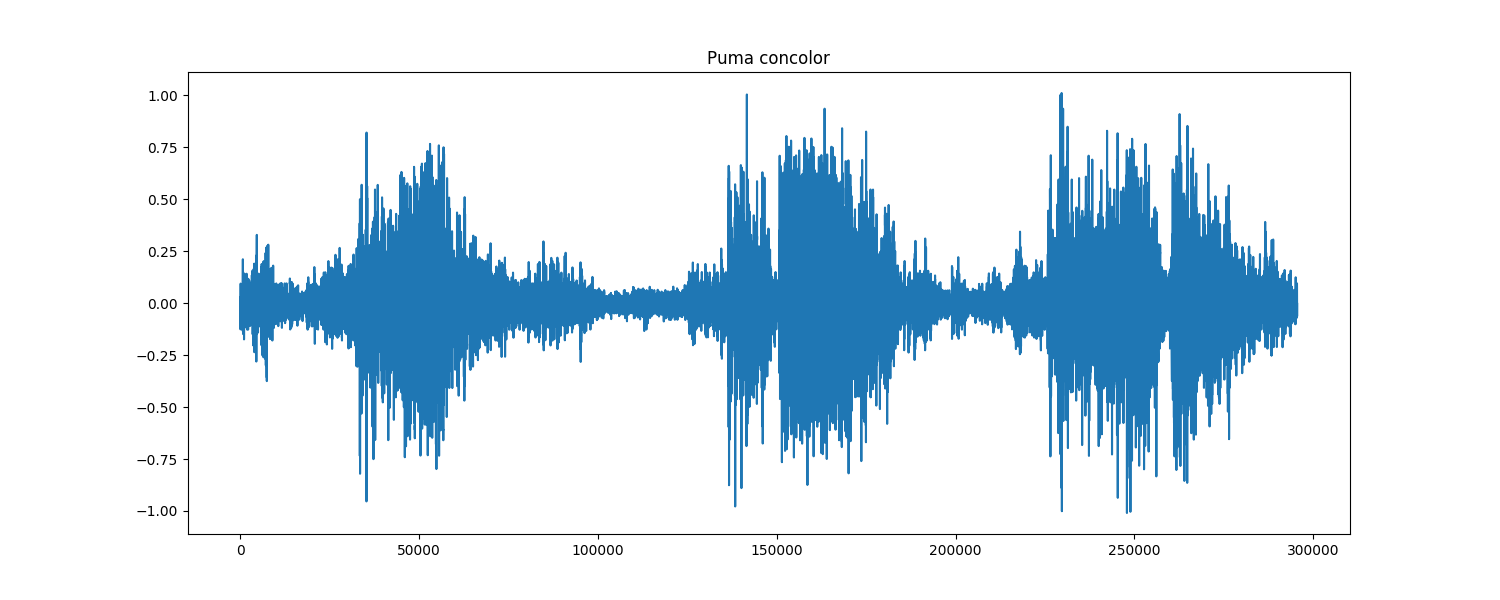
\includegraphics[width=\textwidth]{oscillogram.png}
    \caption{Oscilograma de una vocalización, de 2 segundos de duración, de un individuo de la especie \textit{ovis orientalis aries} (oveja doméstica).}
    \label{img:oscillogram}
\end{figure}

Una importante clase de sonidos son aquellos que consisten en oscilaciones que se repiten periódicamente cada un cierto tiempo.
La duración de una de estas oscilaciones es conocida como su \textit{período} (en segundos) y a la medida inversa se le denomina \textit{frecuencia} (en Hz).
Existen otros sonidos de características aleatorias y que no se repiten periódicamente, llamados \textit{ruidos}.

Una oscilación puede ser descompuesta en una suma de sinusoides elementales de diferentes frecuencias, mediante la aplicación de la \textbf{transformada de Fourier}.
La representación de la transformada de Fourier de una señal en un tiempo dado es conocida como su \textbf{espectro} (figura~\ref{img:spectrum+spectrogram}a).
Esta transformada puede ser igualmente computada sobre pequeñas tramas de tiempo superpuestas, lo que produce una representación tridimensional de la intensidad de las frecuencias en el tiempo, que llamamos \textbf{espectrograma} (figura~\ref{img:spectrum+spectrogram}b).

\begin{figure}[!h]
    \centering
    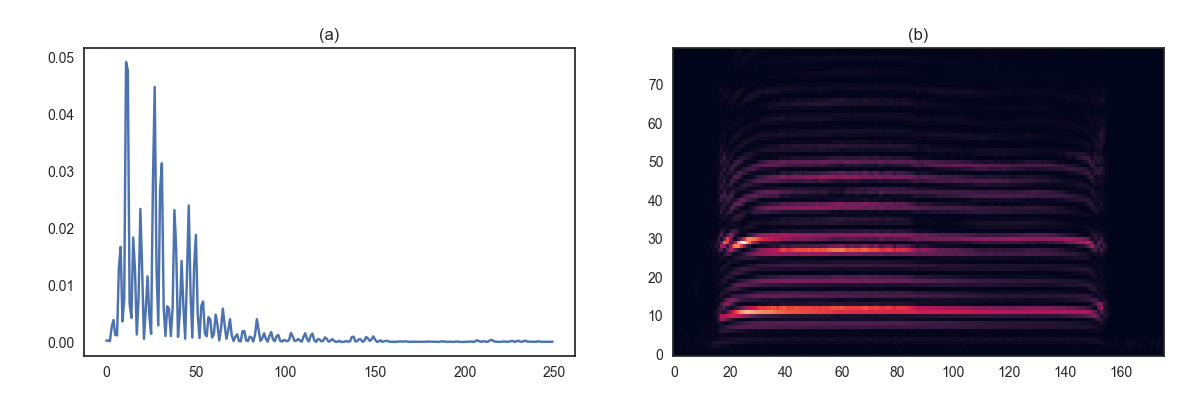
\includegraphics[width=\textwidth]{spectrum+spectrogram.png}
    \caption{Representaciones de la transformada de Fourier de la señal de la figura~\ref{img:oscillogram}: (a) Espectro de una trama. (b) Espectrograma.}
    \label{img:spectrum+spectrogram}
\end{figure}

Para el procesamiento computacional de una señal, esta debe ser llevada del dominio analógico al digital, para lo cual se discretiza mediante observaciones realizadas a intervalos regulares.
Los pasos más importantes en esta conversión de la señal de analógica a digital son:

\begin{enumerate}
    \item \textbf{Filtrado}: La señal analógica se filtra con el propósito de limitar las frecuencias presentes al intervalo $[0,B]$, donde $B$ es la frecuencia \textit{máxima} o \textit{de corte}.
    \item \textbf{Muestreo}: Se digitaliza la señal resultante del paso anterior;
    se emplea \textit{frecuencia de muestreo} $F_s = 2B$ para evita el fenómeno de \textit{aliasing}\footnote{Efecto que causa que señales continuas distintas se tornen indistinguibles cuando se muestrean digitalmente si la tasa de muestreo es menor que el doble de la frecuencia más alta.
    Cuando esto sucede, la señal original no puede ser reconstruida de forma unívoca a partir de la señal digital.}.
    \item \textbf{Cuantificación}: La señal digital es cuantificada, se limita el espacio de almacenamiento ocupado por cada muestra.
\end{enumerate}

Para una calidad de audio de CD se emplean valores de muestreo $F_s = 44.1$ kHz y una cuantificación de 16 bits por muestra.

Los algoritmos de inteligencia artificial tradicionalmente operan con vectores numéricos, llamados \textit{vectores de características}.
En las siguientes secciones analizamos los procedimientos mediante los cuales una señal de audio digital se transforma en una secuencia de tales vectores.

Al procesar una grabación sonora, determinados intervalos de tiempo y/o frecuencias pueden resultar más <<importantes>> que otros.
Estas secciones, conocidas como \textit{segmentos}, permiten establecer una correspondencia entre un evento de sonido y un individuo de una especie dada.
La segmentación, por lo tanto, simplifica la tarea de clasificar una señal acústica;
y las operaciones de procesamiento y extracción de características que se mencionan en lo adelante se aplican sobre dichos segmentos.

\section{Tramas}\label{sec:frames}
Para procesar una señal esta a menudo es dividida en pequeños segmentos, conocidos como \textit{tramas}\footnote{\textit{frames} en inglés.}, de longitud constante y espaciados en intervalos de tiempo iguales.
Denotamos por $N$ la cantidad de muestras de la señal que contiene una trama;
de esta forma la duración de una trama será de $N/F_s$.
Asimismo, denotamos por $M$ la cantidad de muestras en que difieren dos tramas consecutivas, conocida como \textit{tamaño de paso}, y que usualmente es menor que $N$.
A partir de estos valores podemos igualmente calcular la cantidad de muestras que dos tramas consecutivas tienen en común, como $N-M$;
y el número de tramas por segundo (\textit{frame rate}) como $F_s/M$.

Cada trama de $N$ muestras es usualmente obtenida mediante la aplicación de una función \textit{ventana} $w(n)$ a la señal, que es distinta de cero solo si $0\leq n\leq N-1$.
Dada la señal $s[n]$, una trama que comienza en la muestra $m$ es obtenida como

\begin{equation}
    \label{eq:windowing}
    s[n]_m = \begin{cases}
                 s[n + m]w(n) & 0\leq n\leq N-1 \\
                 0 & eoc.
    \end{cases}
\end{equation}

% TODO Move this to a table
Dos de las variantes más conocidas para la función $w(n)$ son las siguientes:

\begin{itemize}
    \item \textbf{Rectangular}:
    \begin{equation*}
        w(n) = \begin{cases}
                   1 & 0\leq n\leq N-1 \\
                   0 & eoc.
        \end{cases}
    \end{equation*}
    \item \textbf{Hamming}:
    \begin{equation*}
        w(n) = 0.53836 - 0.46164 \cos\left(\frac{2\pi n}{N-1}\right)
    \end{equation*}
\end{itemize}

La elección de la ventana $w(n)$ tiene un efecto sobre los resultados de operaciones posteriores sobre las tramas obtenidas.
En la práctica, algunos métodos de procesamiento, como la transformada de Fourier producen mejores resultados cuando se emplean funciones que se aproximan a cero en sus extremos, como la de Hamming.

Una vez computados, los valores asociados a una característica de la señal para cada trama suelen ser <<generalizados>> para representar su comportamiento global.
El procedimiento varía desde la generación de nuevas características a partir de las ya calculadas~\cite{Giret11}, hasta la simplificación de estas a la media y varianza de cada una de sus componentes.
Esto es especialmente importante para el empleo de dichos vectores en algoritmos de inteligencia artificial, puesto que las señales no siempre se descomponen en un mismo número de tramas;
mientras que aplicando este método, el tamaño de los vectores de características sí será igual para todas, lo cual es un requisito de muchos de dichos algoritmos.

\section{Características de bajo nivel de MPEG-7}\label{sec:mpeg7}
MPEG-7 es un estándar para la descripción de contenido multimedia, que define un conjunto de atributos simples y de bajo nivel con el propósito de caracterizar cualquier tipo de sonido.
Este conjunto está constituido por 17 características asociadas a toda señal de sonido~\cite{Kim05,Manjunath02}.
A continuación presentamos una descripción de estas, agrupándolas de acuerdo al modo en que describen la señal.

\subsection{Descriptores básicos}\label{subsec:descriptoresBásicos}

Las dos características de esta categoría describen las propiedades de la señal en el dominio del tiempo de forma simple;
el costo computacional de calcularlas es bajo.

\subsubsection{Audio Waveform}

Para computar esta característica se divide la señal en tramas no superpuestas ($M = N$), y se computan, por cada trama, los 2 valores siguientes:

\begin{itemize}
    \item Menor valor de amplitud de la señal presente en la trama.
    \item Mayor valor de amplitud de la señal presente en la trama.
\end{itemize}

El \textit{audio waveform} (AWF) de la señal consistirá en un vector con los pares calculados, correspondientes a cada una de dichas tramas.

La extracción de esta característica puede ser vista como un modo de <<compresión>> de la señal.
Si se toma $N=1$ se obtendrá la propia señal, mientras que a medida que se seleccionen valores de $N$ más altos, el número de valores resultantes será cada vez menor, obteniéndose una representación reducida de la señal original.
El AWF puede representarse gráficamente como un conjunto de segmentos con extremos en los valores de la tupla correspondiente y desplazados en el tiempo relativo a su posición en la señal (figura~\ref{img:awf+ap}).

\subsubsection{Audio Power}

El \textit{audio power} (AP) describe el comportamiento de la potencia de la señal en cada instante de tiempo.
Al igual que para la AWF, su cálculo requiere dividir la señal en tramas no superpuestas;
y se computa, para la trama $x[n]$ mediante la siguiente expresión:

\begin{equation}
    \label{eq:AP}
    AP = \frac{1}{N}\sum_{n=0}^{N-1}{|x[n]|^2}
\end{equation}

La representación gráfica del AP posibilita el análisis directo de la evolución de la amplitud de la señal en el transcurso del tiempo, lo que puede observarse en la figura~\ref{img:awf+ap}.

\begin{figure}[!h]
    \centering
    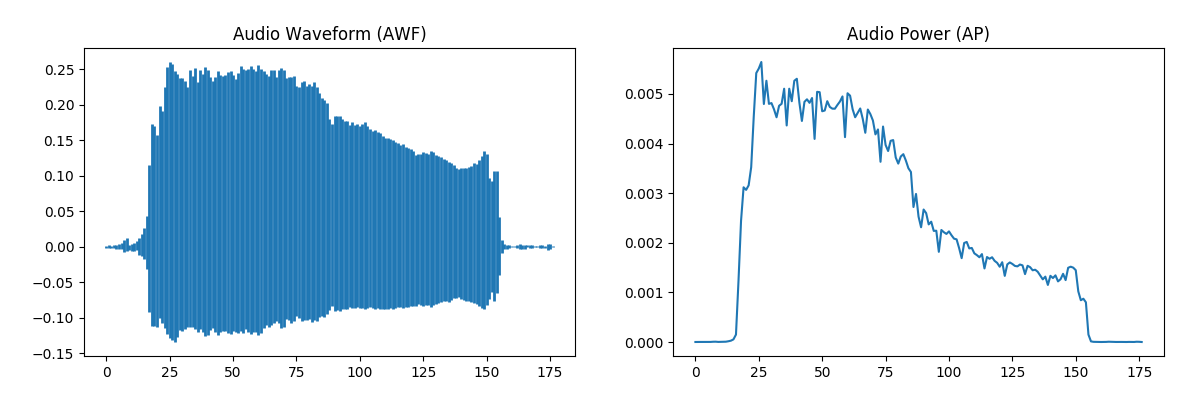
\includegraphics[width=\textwidth]{awf+ap.png}
    \caption{Características básicas de una señal de audio según MPEG-7.}
    \label{img:awf+ap}
\end{figure}



%\section{Representaciones frecuencia-tiempo}\label{sec:representacionesFrecuencia-tiempo}
%El primer paso para el análisis de una señal suele ser su descomposición en frecuencias.
Una trama $x[n]$, de longitud $N$, tiene una representación en dicho dominio que puede ser obtenida mediante la aplicación de la transformada discreta de Fourier (DFT por sus siglas en inglés):

\begin{equation}
    \label{eq:DFT}
    X[f] = \sum_{n=0}^{N-1}{x[n]e^{\frac{-i2\pi fn}{N}}}
\end{equation}

El espectro $X[f]$ puede ser transformado de vuelta al dominio del tiempo aplicando la transformada discreta inversa de Fourier (IDFT):

\begin{equation}
    \label{eq:IDFT}
    x[n] = \frac{1}{N}\sum_{f=0}^{N-1}{X[f]e^{\frac{i2\pi fn}{N}}}
\end{equation}

Al ser $x[n]$ un vector de valores reales, podemos aplicar sobre este una propiedad de la DFT que plantea que el vector $X[f]$ es, por tanto, conjugado simétrico, por lo que suelen considerarse solamente los últimos $\lceil (N+1)/2 \rceil$ valores de este.

Podemos definir $X[f,t]$ como la matriz compuesta por las DFTs correspondientes a cada una de las tramas de una señal, donde el valor en la posición $(f, t)$ corresponde a la amplitud de la frecuencia $f$ en la trama $t$.
A partir de esta matriz se construye el espectrograma de la señal.

%
%\section{Características temporales}\label{sec:característicasTemporales}
%Las características temporales, que describen las propiedades de la señal en el dominio del tiempo, son muy simples;
y se computan directamente a partir de la señal digitalizada.
A continuación se mencionan varias de ellas.

\subsection{Log-Attack Time}\label{subsec:log-attackTime}

El \textit{attack} de una señal se define como el espacio de tiempo, al inicio de esta, en que su intensidad va en ascenso.

El \textit{log-attack time} (LAT)~\cite{Gunasekaran11,Kim05,Manjunath02,Peters04} se calcula entonces como el logaritmo en base 10 de la duración del intervalo de tiempo transcurrido entre los momentos en que la señal se hace audible ($startAttack$) y en que alcanza su máxima intensidad ($stopAttack$):

\begin{equation}
    \label{eq:LAT}
    LAT = \log_{10}{(stopAttack - startAttack)}
\end{equation}

Específicamente, los momentos $stopAttack$ y $startAttack$ suelen definirse como los puntos en que la potencia de la señal alcanza el 20\% y el 90\% de su máximo respectivamente.

\subsection{Audio Waveform}\label{subsec:audioWaveform}

Para computar esta característica se divide la señal en tramas no superpuestas ($M = N$), y se computan, por cada trama, los 2 valores siguientes:

\begin{itemize}
    \item Menor valor de amplitud de la señal presente en la trama.
    \item Mayor valor de amplitud de la señal presente en la trama.
\end{itemize}

El \textit{audio waveform} (AWF)~\cite{Kim05,Manjunath02} de la señal consistirá en un vector con los pares calculados, correspondientes a cada una de dichas tramas.

La extracción del AWF puede ser vista como un modo de <<compresión>> de la señal.
Si se toma $N=1$ se obtendrá la propia señal, mientras que a medida que se seleccionen valores de $N$ más altos, el número de valores resultantes será cada vez menor, obteniéndose una representación reducida de la señal original.
El AWF puede representarse gráficamente como un conjunto de segmentos con extremos en los valores de la tupla correspondiente y ubicados según el momento en que ocurren en la señal (figura~\ref{img:awf+ap}).

\subsection{Audio Power}\label{subsec:audioPower}

El \textit{audio power} (AP)~\cite{Kim05,Manjunath02} describe el comportamiento de la potencia de la señal en cada instante de tiempo.
Al igual que para la AWF, su cálculo requiere dividir la señal en tramas no superpuestas;
y se computa, para la trama $x[n]$ mediante la siguiente expresión:

\begin{equation}
    \label{eq:AP}
    AP = \frac{1}{N}\sum_{n=0}^{N-1}{|x[n]|^2}
\end{equation}

La representación gráfica del AP posibilita el análisis directo de la evolución de la amplitud de la señal en el transcurso del tiempo, lo que puede observarse en la figura~\ref{img:awf+ap}.

\begin{figure}[!h]
    \centering
    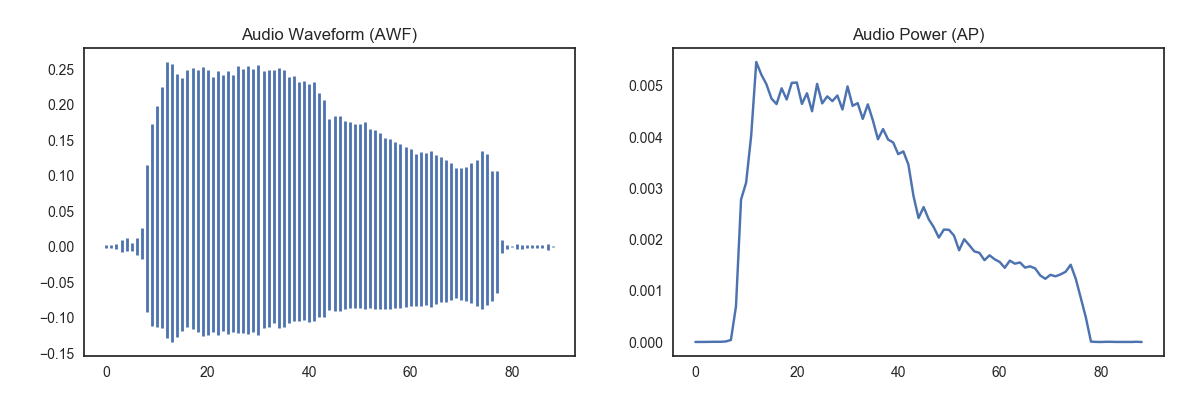
\includegraphics[width=\textwidth]{temporal-features.png}
    \caption{Dos características temporales básicas de una señal de audio: \textit{Audio Waveform} y \textit{Audio Power}, correspondientes a la señal de la figura~\ref{img:oscillogram}.}
    \label{img:awf+ap}
\end{figure}

\subsection{Temporal Centroid}\label{subsec:temporalCentroid}

El \textit{temporal centroid} (TC)~\cite{Kim05,Manjunath02,Peters04,Zamanian17} de la señal es el punto donde se localiza el centro de masas de su AP\@.
Se calcula mediante la siguiente expresión:

\begin{equation}
    \label{eq:TC}
    TC = \frac{\sum_{t=0}^{T-1}{AP_t \cdot t}}{\sum_{t=0}^{T-1}{AP_t}}
\end{equation}

\noindent
donde $T$ es la cantidad de tramas en que se descompuso la señal.

\subsection{Effective Duration}\label{subsec:effectiveDuration}

La \textit{effective duration} (ED)~\cite{Peters04} de una señal constituye la duración del intervalo de tiempo en que esta es perceptible;
el que generalmente se considera como el intervalo en que la amplitud de la señal permanece por encima del 40\% de su valor máximo.

\subsection{Auto-correlation}\label{subsec:auto-correlation}

La \textit{auto-correlation} (AC)~\cite{Gunasekaran11,Peters04} de la señal está dada por un vector de coeficientes que describen su distribución espectral en el dominio del tiempo.
El coeficiente $k$-ésimo se calcula mediante la expresión:

\begin{equation}
    \label{eq:AC}
    AC_k = \frac{1}{x[0]^2}\sum_{n=0}^{N-k-1}{x[n]\cdot x[n+k]}
\end{equation}

\subsection{Zero Crossing Rate}\label{subsec:zeroCrossingRate}

El \textit{zero crossing rate} (ZCR)~\cite{Fagerlund07,Gunasekaran11,Peters04} es una medida del número de veces que la amplitud de la señal cambia de signo.
Los sonidos periódicos tienden a tener un pequeño valor de ZCR, mientras que para los ruidos este valor suele ser alto.

Puede ser computado de forma global, o para cada trama de la señal, aplicando la siguiente expresión:

\begin{equation}
    \label{eq:ZCR}
    ZCR = \frac{1}{2}\sum_{n=1}^{N-1}{|\text{sign}(x[n]) - \text{sign}(x[n-1])|}
\end{equation}

%
%\section{Características espectrales}\label{sec:característicasEspectrales}
%Las características de esta categoría describen la representación de las señales de sonido en el dominio de las frecuencias.

Una trama $x[n]$, de longitud $N$, tiene una representación en el dominio de las frecuencias que puede ser obtenida mediante la aplicación de la \textbf{transformada discreta de Fourier} (DFT por sus siglas en inglés):

\begin{equation}
    \label{eq:DFT}
    X[f] = \sum_{n=0}^{N-1}{x[n]e^{\frac{-i2\pi fn}{N}}}
\end{equation}

El espectro $X[f]$ puede ser transformado de vuelta al dominio del tiempo aplicando la \textbf{transformada discreta inversa de Fourier} (IDFT):

\begin{equation}
    \label{eq:IDFT}
    x[n] = \frac{1}{N}\sum_{f=0}^{N-1}{X[f]e^{\frac{i2\pi fn}{N}}}
\end{equation}

Al ser $x[n]$ un vector de valores reales, podemos aplicar sobre este una propiedad de la DFT que plantea que el vector $X[f]$ es, por tanto, conjugado simétrico, por lo que suelen considerarse solamente los últimos $\lceil (N+1)/2 \rceil$ valores de este.

La posición $k$-ésima del vector $X[k]$ contiene la amplitud correspondiente a la frecuencia $k(F_s/N)$ en la señal.

Podemos definir $X[f,t]$ como la matriz compuesta por las DFTs correspondientes a cada una de las tramas de una señal, donde el valor en la posición $(f, t)$ corresponde a la amplitud de la frecuencia $f$ en la trama $t$.
A partir de esta matriz se construye el espectrograma de la señal.

\subsubsection{Spectral Centroid}

El \textit{spectral centroid} (SC) constituye el centro de masas del espectro de frecuencias de una trama, y permite describir la señal en términos del tipo de frecuencias predominantes (altas o bajas) en cada trama.
Puede computarse mediante la siguiente expresión:

\begin{equation}
    \label{eq:SC}
    SC = \frac{\sum_{k=0}^{K-1}{f(k)|X[k]|}}{\sum_{k=0}^{K-1}{|X[k]|}}
\end{equation}

\noindent
donde $K$ es la longitud del vector correspondiente a la DFT de la trama, y $f(k)$ frecuencia asociada a la posición $k$-ésima de este.

\subsubsection{Spectral Spread}

También conocido como \textit{instantaneous bandwith} o \textit{spectral width}, el \textit{spectral spread} (SS) de una señal refleja la dispersión del espectro de frecuencias en torno a su centroide.

Puede calcularse aplicando la siguiente expresión en cada trama:

\begin{equation}
    \label{eq:SS}
    SS = \sqrt{\frac{\sum_{k=0}^{K-1}{\left[ \log_{2}{(f(k))-SC} \right]^2 |X[k]|}}{\sum_{k=0}^{K-1}{|X[k]|}}}
\end{equation}

\noindent
donde $X[k]$ es la DFT de la trama, y tiene cardinalidad $K$.

Valores bajos (característicos de sonidos armónicos) del SS expresan una concentración de las amplitudes alrededor de la frecuencia centroide;
los valores altos (propios de ruidos), en cambio, muestran una dispersión de las amplitudes en un rango de frecuencias mayor.

\subsubsection{Spectral Roll-off}

El \textit{spectral roll-off} (SRO) se define como la frecuencia bajo la cual se encuentra un porcentaje específico (usualmente entre el 85\% y el 99\%) de la energía espectral total.

\subsubsection{Spectral Flux}

Caracteriza la variación dinámica de la información espectral.
El \textit{spectral flux} (SFX) se calcula como la norma de la diferencia entre los espectros de dos tramas consecutivas.
El coeficiente correspondiente a la trama $t$, $t\geq 1$, puede calcularse entonces aplicando:

\begin{equation}
    \label{eq:SFX}
    SFX_t = ||\hat{X}_t -\hat{X}_{t-1}||
\end{equation}

\noindent
donde $\hat{X}_t$ es la transformada discreta de Fourier de la trama $t$-ésima de la señal.

\subsubsection{Spectral Flatness}

El \textit{spectral flatness} (SF) de una señal refleja su similitud a una señal compuesta por ruido, caso en que su valor se aproxima a 1;
mientras que si se trata de una señal armónica, el valor será próximo a 0.

El SF se calcula como la razón entre las medias geométrica y aritmética de las amplitudes presentes en la DFT de la trama, es decir, mediante la expresión:

\begin{equation}
    \label{eq:SF}
    SF = \frac{\prod_{k=0}^{K-1}{|X[k]|}^{\frac{1}{K}}}{\frac{1}{K}\sum_{k=0}^{K-1}{|X[k]|}}
\end{equation}

\noindent
donde $X[k]$ es la DFT de la trama, de cardinalidad $K$.

\begin{figure}[!h]
    \centering
    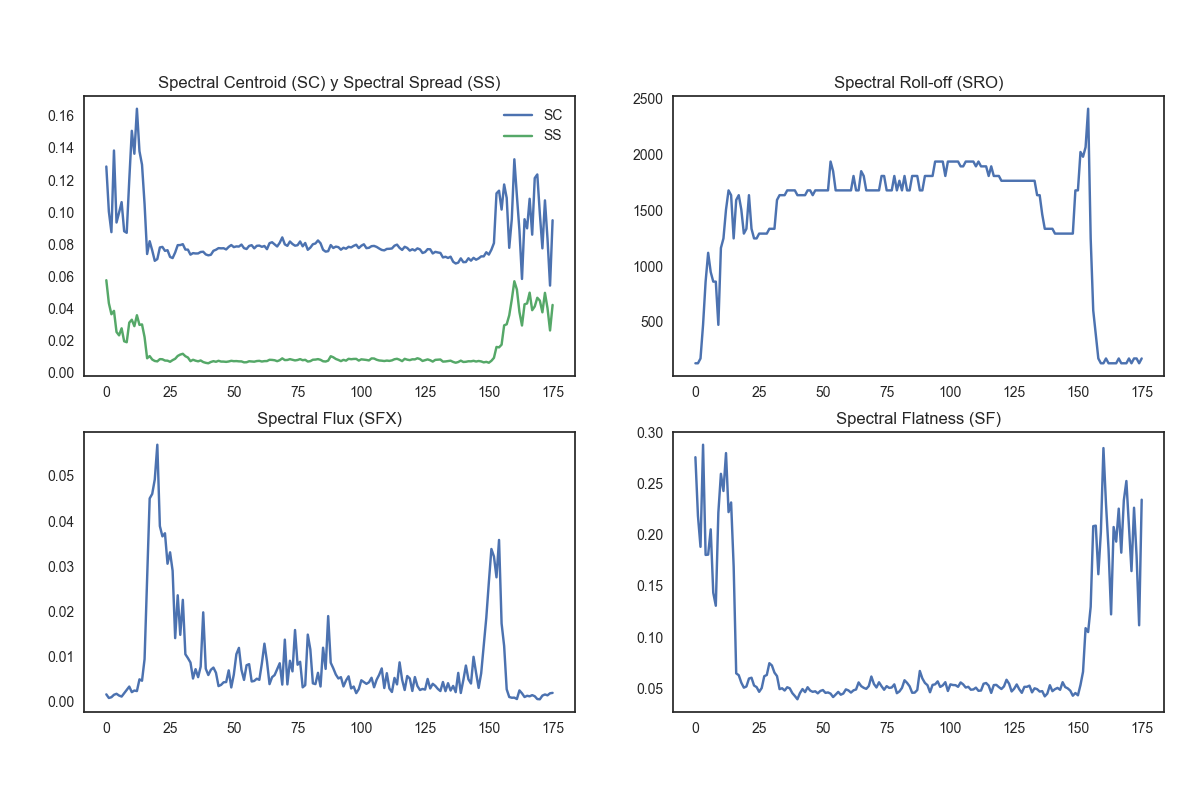
\includegraphics[width=0.95\textwidth]{spectral-features.png}
    \caption{Características espectrales básicas de una señal de audio.}
    \label{img:basic-spectral-descriptors}
\end{figure}

\section{Mel Frequency Cepstral Coefficients}\label{sec:MFCC}
Los \textit{Mel Frequency Cepstral Coefficients} (MFCC)~\cite{Davis80} son coeficientes para la representación del habla basados en la percepción auditiva humana.
Su objetivo es caracterizar el contenido relevante de la señal, obviando aquellas características que poseen información poco valiosa como el ruido de fondo, emociones, volumen, tono, etc.
Si bien fueron desarrollados para tareas asociadas al reconocimiento automático del habla, igualmente han tenido una amplia aplicación en áreas relacionadas al procesamiento de señales musicales y bioacústicas~\cite{McKinney03,Dufour14,Clemins05,Lee06,Li01,Cowling03,Mitrovic06,Fagerlund07}.

Los MFCC se basan en la característica del sistema auditivo humano que provoca que para este sea más difícil discernir entre dos frecuencias cercanas cuanto más altas ellas sean.
La \textbf{escala Mel} (figura~\ref{img:mel-scale}) fue desarrollada con el propósito de representar esta propiedad, permitiendo medir las frecuencias de un modo más acorde a la percepción humana de estas, mediante el uso de la unidad de medida conocida como \textit{Mel}.

\begin{figure}[!h]
    \centering
    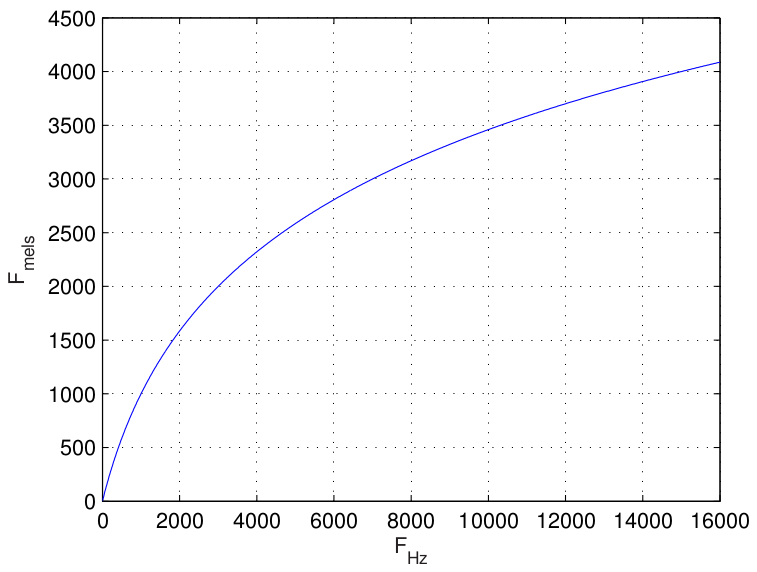
\includegraphics[width=0.5\textwidth]{mel-scale.png}
    \caption{Correspondencia entre las unidades de medida de frecuencias \textit{Hz} y \textit{Mel} de acuerdo con la escala Mel.}
    \label{img:mel-scale}
\end{figure}

La conversión de Hertz ($f$) a Mel ($m$) se realiza aplicando la ecuación~(\ref{eq:Hz-Mel}), mientras que por~(\ref{eq:Mel-Hz}) se puede convertir en sentido contrario.

\begin{equation}
    \label{eq:Hz-Mel}
    m = 2595\log_{10}\left( 1 + \frac{f}{700} \right)
\end{equation}

\begin{equation}
    \label{eq:Mel-Hz}
    f = 700\left( 10^{m/2595} - 1 \right)
\end{equation}

Una ventaja de la escala Mel es que nos permite definir los llamados \textbf{bancos de filtros de Mel}, mediante los cuales podemos <<resumir>> la energía de una señal en $M$ regiones de frecuencias repartidas en correspondencia con la escala Mel (más distanciadas a medida que las frecuencias se hacen mayores).
Para ello, dividimos el intervalo de frecuencias presente en la señal en $M+2$ puntos igualmente distanciados.
A continuación los convertimos a Mel, de forma que ahora estos estarán situados a distancias correspondientes a la percepción humana de las frecuencias.
Luego, definimos los $M$ filtros mediante la siguiente fórmula:

\begin{equation}
    \label{eq:Mel filterbank}
    H_m(k) = \begin{cases}
                 0 & k < f_{m-1} \\
                 \frac{k-f_{m-1}}{f_m - f_{m-1}} & f_{m-1}\leq k\leq f_m \\
                 \frac{f_{m+1}-k}{f_{m+1}-f_m} & f_m \leq k\leq f_{m+1} \\
                 0 & k > f_{m+1} \\
    \end{cases}
\end{equation}

\noindent
donde $f_m$ es la frecuencia correspondiente al $m$-ésimo punto del intervalo.
La representación gráfica de un resultado de la aplicación del procedimiento anterior puede observarse en la figura~\ref{img:mel-filters}.

\begin{figure}[!h]
    \centering
    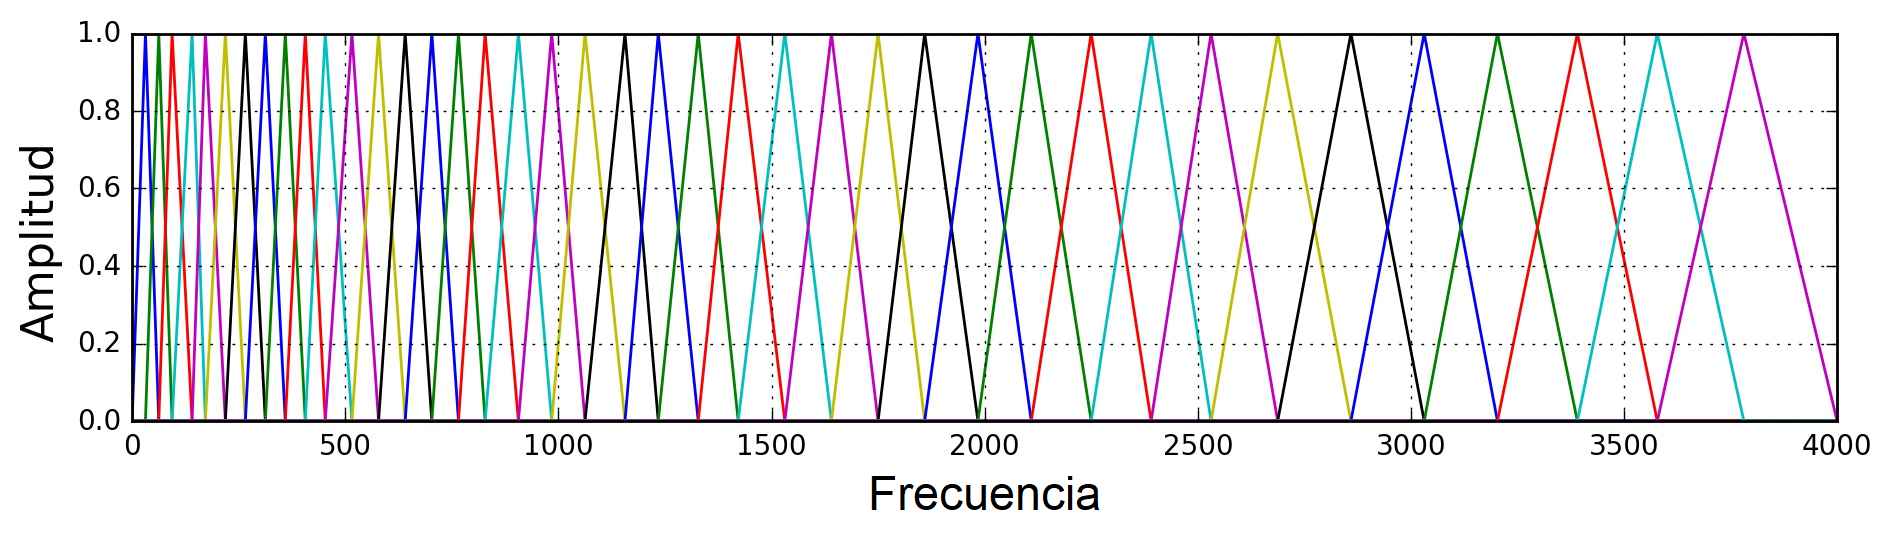
\includegraphics[width=\textwidth]{mel-filters.png}
    \caption{Banco de 40 filtros de Mel en el intervalo de frecuencias de 0~Hz a 4~000~Hz.}
    \label{img:mel-filters}
\end{figure}

A partir de todo lo anterior podemos definir el algoritmo para el cálculo de los MFCC como sigue:

\begin{algorithm}
    \caption{Cálculo de los MFCC}
    \label{algorithm:MFCC}
    Descomponer la señal $s[n]$ en tramas $s[n]_m = x[n]$ aplicando una función ventana\;
    Por cada trama calcular la potencia espectral (periodograma) a partir de su DFT, cuya $k$-ésima componente se calcula mediante la ecuación
    \[
        P[k] = \frac{|X[k]|^2}{K}
    \]
    donde $K$ es la dimensión de la DFT de la trama\;
    Aplicar el banco de filtros de Mel a $P[k]$ y sumar las energías de cada filtro.
    Aplicando $M$ filtros, se obtendrá entonces un vector de $M$ componentes (energías)\;
    Calcular el logaritmo de las energías\;
    Aplicar la transformada de coseno discreta (DCT) al vector de los logaritmos\;
\end{algorithm}

Los pasos del 1 al 4 cumplen la meta de lograr un <<resumen>> de la energía presente en la señal que se corresponda con la percepción humana del sonido.
El paso número 5, persigue eliminar la correlación entre los coeficientes.
Gracias a la aplicación de la DCT, se obtiene un vector de componentes independientes entre sí (no correlacionadas), y por lo tanto este puede ser utilizado en otros procedimientos que así lo requieran.

La DCT se calcula mediante la siguiente ecuación:
\begin{equation}
    \label{eq:DCT}
    f[j] = \sum_{m=0}^{M-1}{e[m]\cos{\left[ \frac{\pi}{M}j\left( m + \frac{1}{2} \right) \right]}}
\end{equation}

Generalmente se usan bancos de entre 20 y 40 filtros y solamente se conservan los primeros 12 o 13 coeficientes;
esto último debido a que la representación obtenida a partir de la aplicación de la DCT suele comprimir la información relevante en los primeros coeficientes, quedando poco valor en los más altos~\cite{Davis80}.

\begin{figure}[!h]
    \centering
    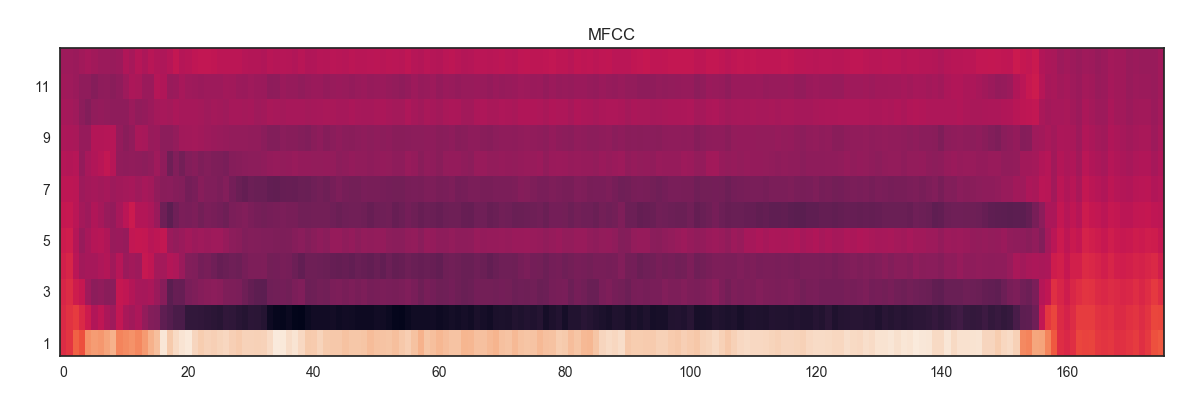
\includegraphics[width=\textwidth]{mfcc.png}
    \caption{Coeficientes MFCC del sonido de la figura~\ref{img:oscillogram}, para tramas de 1024 muestras con un tamaño de paso de 512 y empleando \textit{Hamming} como ventana.}
    \label{img:mfcc}
\end{figure}

Los coeficientes \textbf{delta} y \textbf{delta-delta}, también conocidos como \textit{diferenciales} y \textit{de aceleración} respectivamente,
constituyen una posible mejora al vector de los MFCC.
Estos incluyen información relativa al comportamiento de la energía espectral en el tiempo, que complementa la información estática de una trama que recogen los MFCC.
Para calcular los coeficientes delta aplicamos la siguiente fórmula:

\begin{equation}
    \label{eq:delta}
    d_t = \frac{\sum_{n=1}^{T}{n(c_{t+n} - c_{t-n})}}{2\sum_{n=1}^{T}{n^2}}
\end{equation}

\noindent
donde $d_t$ es el vector de coeficientes delta correspondiente a la trama $t$, y $c_{t+n}$ y $c_{t-n}$ son los MFCC de las tramas posteriores y anteriores respectivamente.
El valor de la cantidad de tramas adyacentes a explorar ($T$) suele ser 2.

Los coeficientes delta-delta pueden ser calculados de igual forma aplicando~(\ref{eq:delta}) empleando los delta en lugar de los MFCC.

A menudo sucede que un segmento de audio está compuesto por más de una trama, de manera que los procedimientos que se han descrito en esta sección producen no un único vector de características sino uno por cada trama del segmento.
Para solucionar esta situación, se construye un único vector con los promedios componente a componente de todos los de la secuencia obtenida~\cite{Lee06,Fagerlund07}.


    %    \chapter{Preprocesamiento de Datos}\label{ch:preprocessing}
    %    % TODO Do this
Lorem ipsum dolor sit amet, consectetur adipiscing elit, sed eiusmod tempor incidunt ut labore et dolore magna aliqua.
Ut enim ad minim veniam, quis nostrud exercitation ullamco laboris nisi ut aliquid ex ea commodi consequat.
Quis aute iure reprehenderit in voluptate velit esse cillum dolore eu fugiat nulla pariatur.
Excepteur sint obcaecat cupiditat non proident, sunt in culpa qui officia deserunt mollit anim id est laborum.



    \chapter{Clustering}\label{ch:clustering}
    Se denominan algoritmos de \textit{clustering} a los algoritmos de aprendizaje no supervisado que agrupan los elementos de un conjunto de datos en conjuntos (clusters) de modo que los objetos pertenecientes a un mismo cluster sean más similares que aquellos en clusters distintos.
Su aplicación permite simplificar la estructura del conjunto de datos, convirtiéndolo en uno más pequeño y fácilmente manipulable;
o como en el caso que ocupa este trabajo, encontrar grupos de especial significación para el problema, como pueden ser agrupaciones de segmentos de audio correspondientes a individuos de una misma especie animal.

% Wikipedia
Los algoritmos de clustering difieren significativamente en su noción de qué constituye un cluster y cómo hallarlos eficientemente.
Algunas de las nociones de cluster más populares incluyen grupos con pequeñas distancias entre sus integrantes, áreas de alta densidad en el espacio de datos, o distribuciones estadísticas particulares.
El algoritmo de clustering más apropiado para un problema, así como su configuración de parámetros (incluyendo la función de distancia a emplear, el umbral de densidad o el número de clusters esperado) es altamente dependiente de las características del conjunto de datos y del uso que se desea dar a los resultados obtenidos.

La determinación del número de conjuntos es a menudo un problema en sí;
algunos algoritmos lo hayan como parte de su funcionamiento, mientras que otros requieren dicho valor como entrada.
A la labor de selección del modelo de <<complejidad>> adecuada se le conoce como \textit{selección del modelo} y las diferentes medidas para la evaluación de los resultados producidos por un modelo dado es un tema que abordamos más adelante en este trabajo.

En las siguientes secciones explicaremos los principales algoritmos de clustering que serán empleados en este trabajo.

\section{Clustering Particional}\label{sec:clusteringParticional}
A continuación es discutido el algoritmo de clustering conocido como K-Means, uno de los más simples y eficientes existentes en la literatura.
Luego de describir en detalle el algoritmo, se analizan algunos de los principales factores que influyen sobre sus resultados.
Finalmente, se presenta una variación de K-Means que busca disminuir la complejidad computacional del algoritmo.

\subsection{K-Means}\label{subsec:k-means}

K-Means~\cite{MacQueen67} es el algoritmo de clustering particional más empleado~\cite{Aggarawal13}.
Comienza seleccionando $K$ puntos representativos como \textit{centroides} iniciales, donde $K$ es un parámetro manualmente especificado por el usuario, siendo este el número deseado de clusters a obtener.
Cada punto del conjunto de datos es luego asignado al centroide más cercano basándose en una medida de proximidad determinada.
Una vez se han formado los clusters, los centroides para cada cluster son actualizados a un nuevo punto.
De manera iterativa, el algoritmo repite estos dos pasos hasta que los centroides no cambien o algún criterio de convergencia alternativo sea cumplido.
K-Means es un algoritmo \textit{greedy} con convergencia garantizada a un mínimo local~\cite{Selim84} pero, visto como un problema de optimización, ha sido demostrado que hallar el mínimo de su función objetivo es NP-Hard~\cite{Manning08}.
En la práctica, suele usarse como criterio de convergencia una versión relajada, continuándose las iteraciones hasta que menos del 1\% de los puntos cambien de cluster.

\begin{algorithm}
    \caption{K-Means}
    \label{algorithm:KMeans}
    Seleccionar $K$ puntos como centroides\;
    \Repeat{Se cumple criterio de convergencia}{
    Formar $K$ clusters asignando cada punto al centroide más próximo\;
    Recomputar el centroide de cada cluster\;
    }
\end{algorithm}

La elección de la medida de proximidad para calcular el centroide más cercano a cada punto puede afectar significativamente las asignaciones y la calidad de la solución final.
Medidas como la distancia Manhattan (norma $L_1$), la distancia euclidiana (norma $L_2$) y la similitud coseno son frecuentemente empleadas, especialmente la segunda.
Tanto la medida de proximidad como el valor de $K$ son determinantes en la configuración de clusters producida por K-Means.

Si se analiza este algoritmo como un problema de optimización, entonces estaría minimizándose la función objetivo de K-Means conocida como \textit{Suma de Errores Cuadráticos} (SSE por sus siglas en inglés), cuya formulación matemática se presenta a continuación.

Dado un conjunto de datos $D={x_1,x_2,\dots,x_N}$ de $N$ puntos, y denotado el conjunto de clusters obtenido tras aplicar K-Means como $C={C_1,C_2,\dots,C_k,\dots,C_K}$;
la SSE para $C$ es definida en la ecuación~(\ref{eq:SSE}) donde $c_k$ es el centroide del cluster $C_k$.

\begin{equation}
    \label{eq:SSE}
    SSE(C)=\sum_{k=1}^{K}{\sum_{x_{i}\in C_k}{dist(x_i, c_k)^2}}
\end{equation}

En otras palabras, se calcula el error de cada punto de los datos, es decir, su distancia al centroide más próximo, y luego es computada la suma de los cuadrados de dichos errores.
Dados dos conjuntos de clusters obtenidos aplicando dos diferentes corridas de K-Means, sería preferible conservar el de menor SSE puesto que esto significaría que los centroides hallados en esa corrida constituyen una mejor representación de los puntos en sus clusters.
De ahí que el resultado de minimizar la función SSE represente el conjunto de clusters óptimo.

Los centroides que minimizan la SSE son la media de los puntos de cada cluster~\cite{Tan05}.
El centroide del $k$-ésimo cluster, $c_k$, quedaría entonces definido según la ecuación~(\ref{eq:centroid}).

\begin{equation}
    \label{eq:centroid}
    c_{k}=\frac{1}{|C_k|}\sum_{x_{i}\in C_k}{x_i}
\end{equation}

Los pasos 3 y 4 del algoritmo~\ref{algorithm:KMeans} directamente intentan minimizar la SSE. El paso 3 forma clusters asignando los puntos al centroide más cercano, lo que minimiza la SSE de dicho conjunto de centroides.
Asimismo, el paso 4 recomputa los centroides, produciendo un nuevo conjunto de menor SSE, en correspondencia con la ecuación ~(\ref{eq:centroid}).
Sin embargo, como se mencionó anteriormente, estos pasos solamente garantizan la convergencia de K-Means a un mínimo local de la función SSE, puesto que la optimizan partiendo de una selección específica de centroides y cantidad de estos, en lugar de todas las posibles opciones.

\subsubsection{Selección de centroides iniciales}

En~\cite{MacQueen67} se propone un simple método de inicialización consistente en seleccionar los $K$ centroides de modo aleatorio.
Este es ampliamente usado en la literatura por su sencillez, aunque tiene la desventaja de que puede producir resultados muy diferentes en varias corridas del algoritmo, algunos de mayor calidad que otros.

Se han popularizado otras variantes de selección de los centroides, con el propósito de aumentar la efectividad y consistencia en los resultados de K-Means.
Uno de ellos es tomar una muestra de puntos y agruparlos empleando una técnica de clustering jerárquico.
Una vez formados $K$ clusters, se toman sus centroides y se inicializa K-Means con estos.
Este enfoque a menudo ofrece buenos resultados, pero solamente resulta práctico si la muestra tomada es relativamente pequeña (de un orden entre $10^2$ y $10^3$) y $K$ es relativamente pequeño comparado con el tamaño de dicha muestra~\cite{Tan05}.

Otra variante, conocida como \textbf{K-Means++}~\cite{Arthur07}, consiste en primeramente seleccionar un punto de manera aleatoria o tomando el centroide de todos los puntos.
Luego, se selecciona el punto más alejado de los centroides formados con anterioridad y se repite este paso hasta obtener $K$ centroides iniciales.

\subsubsection{Estimación del número de clusters}

K-Means es un algoritmo extremadamente dependiente del valor de $K$ seleccionado por el usuario.
La decisión de tal número constituye uno de los mayores desafíos, si no el mayor, al hacer uso de este algoritmo.
Es por esto que numerosos trabajos se han enfocado en el área de determinar el $K$ más apropiado, y varios métodos han sido desarrollados con tal propósito.
A continuación se mencionan algunos de los más generalizados.

\begin{enumerate}
    \item \textbf{Índice de Calinski-Harabasz}~\cite{Calinski74}: Está definido por la ecuación~(\ref{eq:CH}):
    \begin{equation}
        \label{eq:CH}
        CH(K)=\frac{\frac{B(K)}{K-1}}{\frac{W(K)}{N-K}}
    \end{equation}
    donde $N$ representa la cardinalidad del conjunto de datos.
    El número de clusters es seleccionado maximizando la función dada en la ecuación~(\ref{eq:CH}).
    $B(K)$ y $W(K)$ constituyen las sumas de los cuadrados de las distancias intra e inter-cluster respectivamente (dados $K$ clusters).

    \item \textbf{Estadística de Brecha}\footnote{\textit{Gap Statistic} en inglés.}~\cite{Tibshirani01}: En este método se generan $B$ conjuntos de datos que siguen una distribución uniforme en el mismo intervalo que los valores del original.
    Sea $W_{b}^{*}(K)$ la suma de los cuadrados de las distancias intra-cluster del $b$-ésimo conjunto de datos, se plantea entonces la siguiente ecuación:
    \begin{equation}
        Gap(K) = \frac{1}{B} \times\sum_{b}{\log(W_{b}^{*}(K)) - \log(W(K))}
    \end{equation}
    El número de clusters seleccionado es el menor valor de $K$ que satisfaga la ecuación~(\ref{eq:Gap}):
    \begin{equation}
        \label{eq:Gap}
        Gap(K) \geq Gap(K+1) - S_{k+1}
    \end{equation}
    donde $S_{k+1}$ es el valor de la desviación estándar de $\log(W_{b}^{*}(K+1))$.

    \item \textbf{Criterio de Información de Akaike (AIC)}~\cite{Yeung01}: Sea $M$ el número de dimensiones del conjunto de datos, $K$ se calcula a partir de la ecuación~(\ref{eq:AIC}).
    \begin{equation}
        \label{eq:AIC}
        K=argmin_{K}[SSE(K)+2M K]
    \end{equation}

    \item \textbf{Coeficiente de Silueta}\footnote{\textit{Silhouette Coefficient} en inglés.}~\cite{Kaufman90}: Su formulación considera tanto la distancia intra-cluster como la inter-cluster.
    Para un punto dado $x_i$, primero se calcula el promedio de las distancias de este a todos los puntos del mismo cluster ($a_i$).
    Luego por cada cluster que no contiene a $x_i$, se computa el promedio de las distancias de $x_i$ a sus integrantes ($b_i$).
    Usando estos dos valores, se estima el coeficiente de silueta de un punto como el cociente entre su diferencia y el mayor de ambos.
    El promedio de todos los coeficientes en el conjunto de datos puede ser empleado para evaluar la calidad de un clustering.
    Mayores valores se corresponden con modelos cuyos clusters se encuentran mejor definidos.
    \begin{equation}
        S = \frac{\sum_{i=1}^{N}{\frac{b_{i}-a_{i}}{\max(a_i,b_i)}}}{N}
    \end{equation}
\end{enumerate}

\subsubsection{Complejidad espacial y temporal}

Los requerimientos de espacio de memoria para K-Means son relativamente pequeños puesto que solamente los puntos y los centroides son almacenados por el algoritmo.
Específicamente, la cantidad de memoria empleada es $O((n+K)m)$, donde $n$ es el número de puntos y $m$ la cantidad de atributos (dimensionalidad) de estos.
Los requisitos de tiempo de este algoritmo son igualmente bajos, es básicamente lineal respecto al tamaño del conjunto de datos.
En particular, el tiempo requerido es $O(I \cdot K \cdot m \cdot n)$, donde $I$ es el número de iteraciones necesarias para converger.
A menudo $I$ es suficientemente pequeño, y usualmente puede ser considerado como un valor constante y despreciable.
De esta forma, K-Means es lineal respecto al tamaño del conjunto de datos $n$, y es muy eficiente siempre que el número de clusters $K$ sea significativamente menor que $n$~\cite{Tan05}.

\subsection{Mini-batch K-Means}\label{subsec:miniBatchKMeans}

Mini-batch K-Means es una variante del algoritmo K-Means que emplea \textit{mini-batches} con el fin de reducir el tiempo de computación, sin afectar la función objetivo a optimizar.
Los \textit{mini-batches} son subconjuntos del conjunto de datos sobre el que se aplica el algoritmo, tomados mediante un muestreo aleatorio en cada iteración.
Estos reducen drásticamente la cantidad de cómputo necesario para converger a un óptimo local.

\begin{algorithm}
    \caption{Mini-batch K-Means}
    \label{algorithm:MiniBatchKMeans}
    Seleccionar $K$ puntos como centroides\;
    \Repeat{Se cumple criterio de convergencia}{
    Tomar una muestra aleatoria de $b$ puntos del conjunto de datos\;
    Asignar cada punto de la muestra al cluster que corresponda al centroide más próximo\;
    Recomputar el centroide de cada cluster\;
    }
\end{algorithm}

Al recomputar los centroides durante cada iteración se tienen en cuenta tanto los puntos de la muestra recién asignados como los asignados durante las iteraciones anteriores.

El algoritmo Mini-batch K-Means converge a mayor velocidad que K-Means, aunque la calidad de sus resultados es menor.
No obstante, para aplicaciones prácticas, esta diferencia en calidad suele ser poco significativa~\cite{Sculley10}.

\section{Clustering Jerárquico Aglomerativo}\label{sec:clusteringJerárquicoAglomerativo}
Las técnicas de clustering jerárquico son, como las de clustering particional, relativamente antiguas en comparación con muchas otras que analizaremos más adelante.
Aún así se mantienen entre las más usadas en la actualidad.
Fueron desarrolladas con la finalidad de resolver algunas de las desventajas de los algoritmos de clustering particional que hemos visto, como su necesidad de una cantidad de clusters prefijada y su naturaleza no determinista.


\section{Clustering Basado en Densidad}\label{sec:Dbscan}
Algoritmos como K-Means presentan dificultades para identificar clusters cuando las distancias entre elementos de un mismo conjunto es mayor que la de elementos de conjuntos distintos.
En estos casos, puesto que K-Means busca minimizar la distancia entre los elementos dentro de un mismo cluster, producirá clusters que difieran significativamente de los grupos <<correctos>>.
Podemos observar un ejemplo en el escenario de la figura~\ref{img:kmeans-dbscan}, donde se compara el resultado de K-Means con el del algoritmo que analizamos en esta sección, conocido como \textit{DBSCAN}.

\begin{figure}[!h]
    \centering
    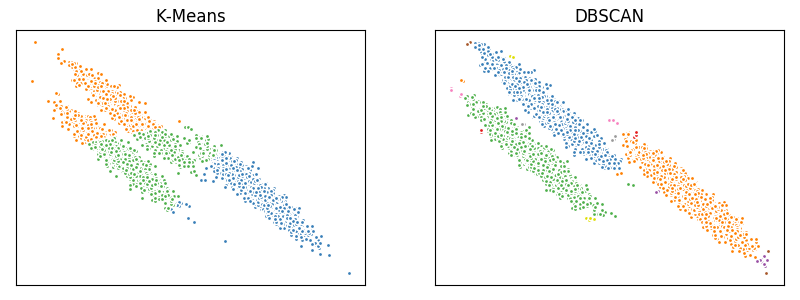
\includegraphics[width=\textwidth]{kmeans-dbscan.png}
    \caption{Resultados de los algoritmos K-Means y DBSCAN ejecutados sobre un conjunto de datos que sigue una distribución anisotrópica.}
    \label{img:kmeans-dbscan}
\end{figure}

En la imagen podemos observar asimismo el comportamiento de otro algoritmo sobre el mismo conjunto de datos.
En esta sección abordamos el algoritmo en cuestión, denominado \textit{DBSCAN}~\footnote{Siglas en inglés de \textit{Density-based spatial clustering of applications with noise}.}, que forma parte del conjunto de algoritmos de clustering basados en la densidad de los datos.

Un cluster basado en el criterio de densidad de los puntos consiste en un área densa de puntos conectados, separado de otros clusters por áreas de menor densidad.

\subsection{Densidad}\label{subsec:densidad}

El algoritmo DBSCAN define la densidad alrededor de un punto como la cantidad de puntos localizados alrededor de este en un radio, $Eps$, específico.
El propio punto es incluido en este conteo.
En la figura~\ref{img:dbscan} se puede observar gráficamente esta definición.
En este caso número de puntos alrededor de $A$ es 7.

El valor del radio es determinante en la densidad de un punto.
Si este valor es suficientemente grande, entonces todos los puntos tendrán una densidad de $n$, el número de puntos en el conjunto de datos.
En cambio, si el radio es demasiado pequeño, la densidad de todos los puntos será igual a 1.
Más adelante discutiremos algunas estrategias para la selección de valores apropiados para el radio.

\begin{figure}[!h]
    \centering
    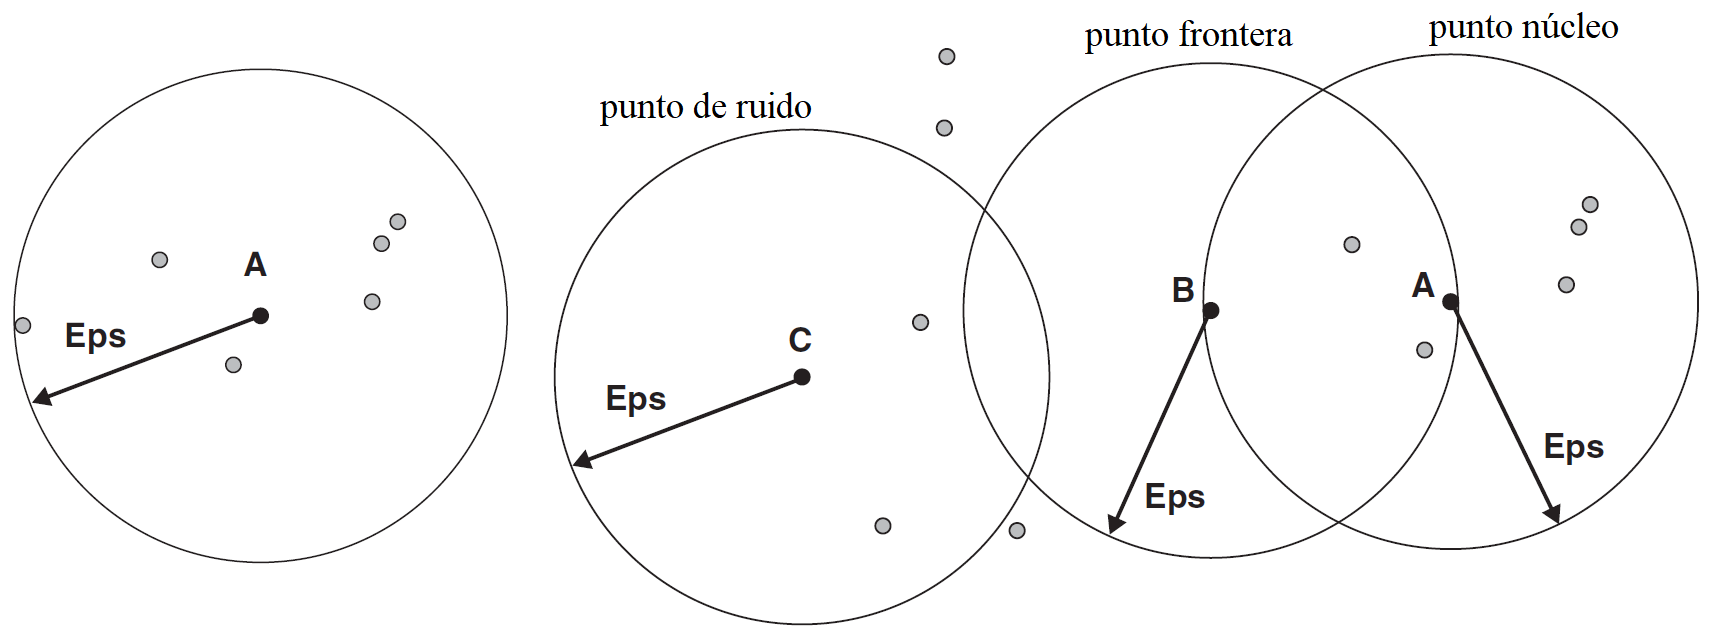
\includegraphics[width=\textwidth]{dbscan.png}
    \caption{Densidad en el entorno de un punto y clasificaciones de los puntos según su densidad. (Tomado de~\cite{Tan05}.)}
    \label{img:dbscan}
\end{figure}

De acuerdo con la densidad de un punto, estos pueden ser clasificados de la siguiente forma:

\begin{itemize}
    \item \textbf{Puntos núcleo}: Constituyen puntos de la región interna de un cluster basado en densidad.
    Un punto es núcleo si el número de puntos alrededor de este (incluyéndolo) supera o iguala un valor $MinPts$, especificado por el usuario.
    En la figura~\ref{img:dbscan} los puntos identificados con la letra $A$ son núcleos para el radio $Eps$ indicado si $MinPts\leq 7$.
    \item \textbf{Puntos frontera}: Un punto frontera es aquel que no cumple el criterio de núcleo, pero que forma parte de la vecindad de al menos uno de estos.
    En la figura~\ref{img:dbscan} $B$ es un punto frontera.
    \item \textbf{Puntos de ruido}: Un punto es de ruido si no es núcleo o frontera.
    En la figura~\ref{img:dbscan} $C$ es un punto de ruido.
\end{itemize}

\subsection{Algoritmo DBSCAN}\label{subsec:algoritmoDbscan}

A partir de las definiciones dadas de puntos núcleos, fronteras y de ruido, podemos describir el algoritmo DBSCAN del siguiente modo: Todo par de puntos núcleos cuya distancia sea no mayor que $Eps$ son asignados al mismo cluster.
De igual forma, los puntos fronteras son asignados al cluster de los puntos núcleos cuya distancia a estos sea menor o igual que $Eps$.
(En caso de estar en la vecindad de núcleos pertenecientes a clusters diferentes, un criterio específico debe ser determinado al programar el algoritmo).
Los puntos de ruido son descartados y no asignados a ningún cluster.

\begin{algorithm}
    \caption{DBSCAN}
    \label{algorithm:DBSCAN}
    Etiquetar todos los puntos como núcleo, frontera o ruido\;
    Eliminar los puntos de ruido\;
    Añadir una arista entre todo par de puntos núcleos que se encuentren a una distancia menor o igual que $Eps$\;
    Convertir cada componente conexa del grafo resultante en un cluster\;
    Asignar cada punto frontera a uno de los clusters de los puntos núcleos asociados a este\;
\end{algorithm}

\subsubsection{Complejidad espacial y temporal}

El algoritmo DBSCAN demora en ejecución un tiempo $O(n \cdot$ tiempo para encontrar puntos en una $Eps$-vecindad), donde $n$ es el número de puntos en el conjunto de datos.
En el peor caso, esta complejidad sería $O(n^2)$.
Sin embargo, el uso de determinadas estructuras de datos en espacios de pocas dimensiones, permite la recuperación eficiente de todos los puntos en un intervalo dado alrededor de un punto específico~\cite{Tan05};
en estos escenarios la complejidad puede llegar a ser $O(n\log n)$.
Los requerimientos de memoria de DBSCAN, aun en espacios de grandes dimensiones, son $O(n)$, puesto que solo es necesario mantener poca información relativa a cada punto, como puede ser el cluster al que pertenece, la clasificación, etc.
No obstante, este uso de memoria depende igualmente del comportamiento de la estructura de datos empleada para computar las vecindades.

\subsubsection{Selección de parámetros para DBSCAN}

Un criterio para determinar los parámetros es mediante la observación del comportamiento de la distancia de los puntos a su $k$-ésimo vecino más cercano, conocida como $k$-distancia.
Si un punto pertenece a un cluster, entonces su $k$-distancia debe ser un valor relativamente pequeño, siempre que $k$ no sea mayor que el tamaño del cluster.
Siempre que las densidades de los clusters no difieran radicalmente, en promedio, los valores de la $k$-distancias para puntos que pertenezcan a algún cluster no mostrarán un rango de valores muy amplio.
En cambio, para puntos que no pertenezcan a ningún cluster, es decir, de ruido, este valor sí estará situado muy por encima del rango antes mencionado.
De esta forma, si tomamos todos los puntos de un conjunto de datos, los ordenamos por su $k$-distancia y estas las representamos en una gráfica, deberíamos obtener una imagen donde existirá un punto de inflexión que se corresponda con el valor de la $k$-distancia a partir del cual los puntos se encuentran fuera de algún cluster.
Podemos entonces tomar dicho valor como el $Eps$ adecuado para el problema en cuestión.
En cuanto al valor de $MinPts$, este sería precisamente el $k$ seleccionado para calcular las distancias, pues los puntos cuya $k$-distancia sea menor que $Eps$ serán etiquetados como núcleos, mientras los demás serán fronteras o ruido.

% TODO Consider putting an example of graphic here

Es importante notar que el valor de $Eps$ resultante de este proceso dependerá del $k$ seleccionado al inicio.
Si $k$ es demasiado pequeño, algunos puntos de ruido situados muy próximos entre sí pudieran ser etiquetados incorrectamente como clusters.
Por otra parte, si $k$ es demasiado grandes, aquellos clusters cuya cantidad de elementos sea menor que $k$ no serán identificados correctamente.

Un defecto del algoritmo DBSCAN es que requiere que las densidades de los clusters (y del espacio de datos en general) muestren comportamientos semejantes.
Un ejemplo de esta afirmación podemos observarlo en la figura~\ref{img:density-issues}.
El ruido alrededor de los clusters $A$ y $B$ presenta la misma densidad que los clusters $C$ y $D$.
Si seleccionamos un $Eps$ suficientemente bajo para detectar a $C$ y $D$, sucederá entonces que $A$, $B$ y el ruido a su alrededor constituirán un mismo cluster.
En cambio si el $Eps$ es tan alto como para distinguir a $A$ y $B$ como clusters independientes, entonces los puntos que forman parte de $C$ y $D$ serán considerados ruido.

\begin{figure}[!h]
    \centering
    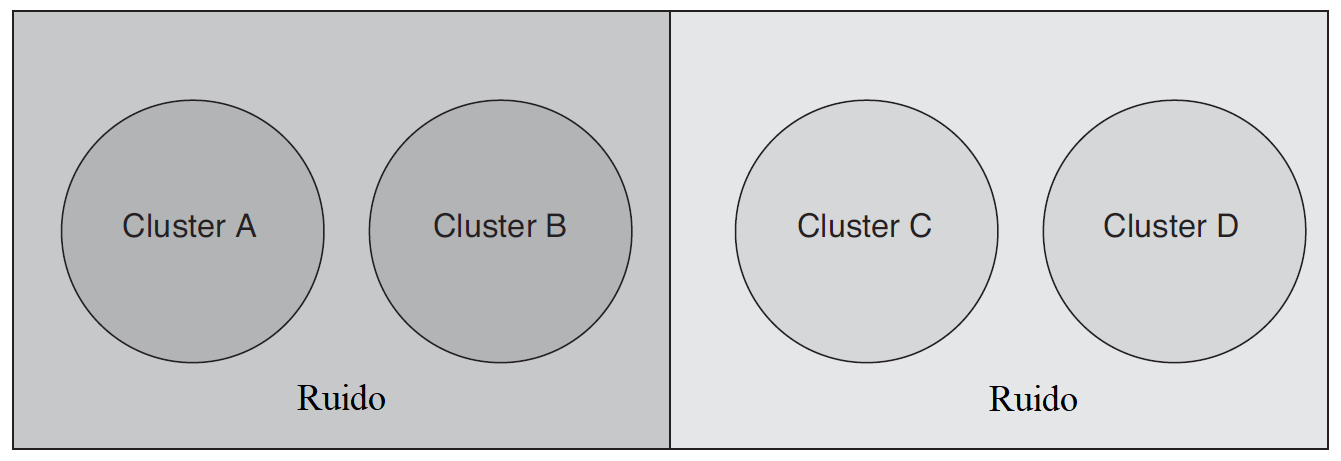
\includegraphics[width=\textwidth]{density-issues.png}
    \caption{Cuatro clusters en un entorno de ruido.
    Los tonos de gris más oscuros indican mayores densidades. (Tomado de~\cite{Tan05}.)}
    \label{img:density-issues}
\end{figure}

% TODO Consider adding HDBSCAN

\section{Clustering Espectral}\label{sec:clusteringEspectral}
% TODO Do it!

\section{Clustering Basado en Probabilidades}\label{sec:clusteringBasadoEnProbabilidades}
Los algoritmos de clustering probabilísticos modelan el conjunto de datos a partir de la asunción de que este es generado mediante la combinación de determinadas distribuciones de probabilidad.
Estos algoritmos transforman el problema de clustering en el de estimar los parámetros para $K$ distribuciones de probabilidad.
Luego los puntos del conjunto de datos que se correspondan con una misma distribución se asociarán al mismo cluster.

En esta sección se analiza un modelo de clustering probabilístico ampliamente estudiado, conocido como \textit{Gaussian Mixture Model} (GMM);
así como la técnica \textit{Expectation-maximization}, empleada para estimarlo computacionalmente.

\subsection{Combinación de modelos}\label{subsec:mixtureModels}

Sea $X={x_1,\dots,x_N}$ un conjunto de datos de $N$ observaciones de una variable aleatoria $x$ con $D$ dimensiones.
Se asume que la variable $x_i$ sigue una distribución consistente con la combinación de $K$ \textbf{distribuciones componentes} (clusters), cada una instancia de una distribución para determinados parámetros.
Puede definirse entonces la función de densidad de $x_i$ como:

\begin{equation}
    \label{eq:mixtureModels}
    p(x_i)=\sum_{k=1}^{K}{\pi_k p(x_i|\theta_k)}
\end{equation}

\noindent
donde cada $\theta_k$ es el conjunto de parámetros específicos de la $k$-ésima componente y $p(x_i|\theta_k)$ su función de densidad.
Los pesos $\pi_k$, también conocidos como \textit{mixing probabilities}, deben satisfacer las condiciones $0\leq \pi_k \leq 1$ y $\sum_{k=1}^{K}{\pi_k}=1$.

Si bien la definición no establece ninguna restricción en cuanto al tipo de distribución que debe seguir cada componente;
en la práctica, para simplificar el estudio de estos modelos, suele asociarse una misma distribución a todas las componentes, variando únicamente sus parámetros.

\subsection{Gaussian Mixture Model}\label{subsec:GMM}

El modelo de clustering probabilístico más extendido es el de combinación de distribuciones normales, conocido en la literatura como \textit{Gaussian Mixture Model} (GMM)~\cite{Murphy12}.
Es asimismo, uno de los modelos de mayor uso en aplicaciones relacionadas con el análisis acústico~\cite{Kakar13,Kwan06,Lee08,Somervuo06,Virtanen18}.

La distribución normal, en el caso de una variable unidimensional $x$, tiene una función de densidad de la forma:

\begin{equation}
    \label{eq:singleGaussian}
    \mathcal{N}(x|\mu,\sigma^2)=\frac{1}{(2\pi\sigma^2)^{1/2}}\exp{(-\frac{1}{2\sigma^2}((x-\mu)^2)}
\end{equation}

\noindent
donde $\mu$ es la media y $\sigma^2$ la varianza.
Para el caso de $D$ dimensiones, la función toma la forma:

\begin{equation}
    \label{eq:multidimGaussian}
    \mathcal{N}(x|\mu,\Sigma)=\frac{1}{(2\pi)^{D/2}|\Sigma|^{1/2}}\exp{(-\frac{1}{2}(x-\mu)^T \Sigma^{-1}(x-\mu))}
\end{equation}

\noindent
donde $\mu$ es el vector $D$-dimensional de medias y $\Sigma$, de dimensión $D\times D$, la matriz de covarianza con determinante $|\Sigma|$.

En GMM cada componente corresponde a una distribución normal con determinados valores asociados a sus parámetros $\mu$ y $\Sigma$.
A partir de la ecuación~(\ref{eq:mixtureModels}) se puede entonces formular este modelo como:

\begin{equation}
    \label{eq:GMM}
    p(x_i|\Theta) = p(x_i|\pi,\mu,\Sigma)= \sum_{k=1}^{K}{\pi_k \mathcal{N}(x_i|\mu_k,\Sigma_k)}
\end{equation}

Para estimar los parámetros de un modelo, puede emplearse el método de máxima verosimilitud.
Dado un conjunto de observaciones $X$, la función de log-verosimilitud se define como:

\begin{equation}
    \label{eq:log-likelihood}
    l(\Theta|X) = \log{p(X|\Theta)} = \sum_{i=1}^{N}{\log{p(x_i|\Theta)}} = \sum_{i=1}^{N}{\log{\sum_{k=1}^{K}{\pi_k \mathcal{N}(x_i|\mu_k,\Sigma_k)}}}
\end{equation}

El método de máxima verosimilitud estima $\Theta$ como el valor que maximiza~(\ref{eq:log-likelihood}).
Para encontrar dicho valor, se pueden computar las derivadas parciales de~(\ref{eq:log-likelihood}) respecto a $\pi_k$, $\mu_k$, y $\Sigma_k$ respectivamente.
Si se iguala a cero la derivada respecto a $\mu_k$, puede despejarse la siguiente expresión:

\begin{equation}
    \label{eq:mu_k}
    \mu_k = \frac{\sum_{i=1}^{N}{\gamma(z_{ik})x_i}}{\sum_{i=1}^{N}{\gamma(z_{ik})}}
\end{equation}

\noindent
donde

\begin{equation}
    \label{eq:gamma}
    \gamma(z_{ik}) = \frac{\pi_k \mathcal{N}(x_i|\mu_k,\Sigma_k)}{\sum_{j=1}^{K}{\pi_j \mathcal{N}(x_i|\mu_j,\Sigma_j)}}
\end{equation}

$\gamma(z_{ik})$ es conocida como la \textbf{responsabilidad} de la componente $k$ sobre la observación $i$-ésima $x_i$.

De igual forma, igualando a cero la derivada de~(\ref{eq:log-likelihood}) respecto a $\Sigma_k$, se obtendrá

\begin{equation}
    \label{eq:Sigma_k}
    \Sigma_k = \frac{\sum_{i=1}^{N}{\gamma(z_{ik})(x_i-\mu_k)(x_i-\mu_k)^T}}{\sum_{i=1}^{N}{\gamma(z_{ik})}}
\end{equation}

Luego de aplicar algunas operaciones adicionales~\cite{Aggarawal13} debido a las características de las restricciones a las que están sujetos los pesos $\pi_k$, se llega a

\begin{equation}
    \label{eq:pi_k}
    \pi_k = \frac{\sum_{i=1}^{N}{\gamma(z_{ik})}}{N}
\end{equation}

Sin embargo, la optimización de la función~(\ref{eq:log-likelihood}) presenta serios inconvenientes debido a la dependencia existente entre las responsabilidades $\gamma(x_{ik})$ y el resto de los parámetros, por lo que no resulta simple derivar una expresión que permita calcular directamente dichos valores.
Generalmente solo pueden ser obtenidos mínimos locales aplicando algoritmos de descenso por gradiente sobre~(\ref{eq:log-likelihood}), lo que igualmente resulta difícil debido a las restricciones del modelo (matriz de covarianzas definida positiva, suma de los pesos $\pi_k$ igual a uno, etc)~\cite{Aggarawal13,Murphy12}.

\subsection{Algoritmo Expectation-maximization}\label{subsec:EM}

El algoritmo \textit{Expectation-maximization} (EM) permite estimar parámetros de máxima verosimilitud para un modelo.
Sigue un proceso iterativo que alterna dos etapas: se infieren valores para los parámetros (\textit{expectation}), y luego se optimizan dichos valores para el conjunto de datos dado (\textit{maximization}).

En el caso particular de GMM, se puede aplicar empleando para ello las ecuaciones obtenidas en la sección~\ref{subsec:GMM} como se explica en el algoritmo~\ref{algorithm:EM}.

\begin{algorithm}
    \caption{Expectation-maximization para GMM}
    \label{algorithm:EM}
    Inicializar $\mu_k^0$, $\Sigma_k^0$, y $\pi_k^0$\;
    \Repeat{Se cumple criterio de convergencia}{
    \textbf{Expectation}: Calcular las responsabilidades $\gamma(z_{ik})$ sustituyendo los valores actuales de los parámetros en~(\ref{eq:gamma})\;
    \textbf{Maximization}: Actualizar los parámetros sustituyendo las responsabilidades actuales en las expresiones (\ref{eq:mu_k}), (\ref{eq:Sigma_k}) y (\ref{eq:pi_k}).
    Las nuevas medias son usadas al calcular las covarianzas\;
    }
\end{algorithm}

Usualmente se toma como criterio de convergencia para este algoritmo que la variación de la log-verosimilitud respecto a la iteración anterior haya sido menor que un valor $\epsilon$ determinado, o se haya superado una cantidad máxima de iteraciones.

La cantidad de iteraciones requeridas por EM para converger es mayor que las que toma K-Means~\cite{Park09}.
Para acelerar la ejecución del algoritmo, generalmente se realiza una corrida de K-Means sobre el conjunto de datos, y se toman las medias, varianzas y proporción de puntos en los clusters para inicializar los parámetros $\mu_k^0$, $\Sigma_k^0$ y $\pi_k^0$ respectivamente.

De forma similar a lo que ocurre con el algoritmo K-Means, EM puede caer en máximos locales en dependencia de los valores iniciales.

\subsubsection{Estimación de hiper-parámetros}

El número de componentes es decisivo en la calidad del resultado producido por el algoritmo EM\@.
Asimismo, debe decidirse cuál emplear entre los diferentes patrones existentes para representar la matriz de covarianza del modelo, mencionados a continuación:

\begin{itemize}
    \item \textbf{Full}: De dimensión $K\times m\times m$.
    Cada componente posee su propia matriz de covarianza.
    \item \textbf{Tied}: De dimensión $m\times m$.
    Todas las componentes comparten la misma matriz de covarianza.
    \item \textbf{Diagonal}: De dimensión $K\times m$.
    Cada componente posee su propia matriz de covarianza diagonal.
    \item \textbf{Spherical}: De dimensión $K\times 1$.
    Cada componente tiene un único valor de varianza que le es propio.
\end{itemize}

A continuación se mencionan dos criterios ampliamente usados para la evaluación de la calidad de un GMM con parámetros calculados aplicando este algoritmo.
Estos facilitan la decisión de los hiper-parámetros en correspondencia con el problema que se intenta modelar.

\begin{enumerate}
    \item \textbf{Criterio de Información de Akaike} (AIC)~\cite{Akaike74}:
    Penaliza la cantidad de parámetros en el modelo, mediante la fórmula
    \begin{equation*}
        AIC = \log(\hat{L}) - d
    \end{equation*}
    donde $d$ es el número de parámetros libres del modelo, y $\hat L$ el valor de la función de log-verosimilitud asociada.
    \item \textbf{Criterio de Información Bayesiano} (BIC)~\cite{Schwarz78}: Al igual que AIC penaliza la complejidad del modelo, aunque en este caso la penalización es mayor.
    Su fórmula es
    \begin{equation*}
        BIC = \log(\hat{L}) - \frac{d}{2}\log(n)
    \end{equation*}
\end{enumerate}

Como se puede apreciar, ambos criterios se basan en la penalización de la función de verosimilitud (log-verosimilitud) a partir de la complejidad del modelo.
De esta forma a modelos más complejos corresponde mayor penalización, y se logra así un equilibrio entre la calidad del resultado y la complejidad del modelo correspondiente.

Se consideran \textit{parámetros libres} aquellos parámetros del modelo estimados aplicando el método de máxima verosimilitud.
Para GMM son $\mu_k$, $\Sigma_k$ y $\pi_k$, que se cuantifican (valor asociado a $d$) por la cantidad total de valores que estos vectores contienen.

\subsubsection{Complejidad espacial y temporal}

El análisis de los requerimientos de memoria de Expectation-maximization no difiere sustancialmente del de K-Means.
Solamente los puntos del conjunto de datos y las variables deben ser almacenados para la ejecución del algoritmo.
No obstante, a diferencia de K-Means donde la única variable asociada al algoritmo era la posición de los centroides, en EM el espacio de memoria ocupado es mayor, principalmente a causa de la matriz de covarianza.
Las dimensiones de esta última varían en dependencia del modo en que sea analizada la covarianza, ya sea individual para cada componente o global, pudiendo ir desde $O(K)$ hasta $O(K \cdot m^2)$.
En el caso peor, la cantidad de memoria es por tanto $O(nm + K \cdot m^2)$.

El tiempo requerido por el algoritmo es igualmente $O(I\cdot K\cdot m\cdot n)$, siendo $I$ el número de iteraciones necesarias para la convergencia. La principal diferencia en este caso radica en el hecho de la cantidad de iteraciones ejecutadas por el algoritmo, que es distinta a la de K-Means, y puede llegar a ser un valor considerablemente elevado~\cite{Firdaus15,Park09}.



    %    \chapter{Evaluación del Clustering}\label{ch:evaluation}
    %    % TODO Do this
Lorem ipsum dolor sit amet, consectetur adipiscing elit, sed eiusmod tempor incidunt ut labore et dolore magna aliqua.
Ut enim ad minim veniam, quis nostrud exercitation ullamco laboris nisi ut aliquid ex ea commodi consequat.
Quis aute iure reprehenderit in voluptate velit esse cillum dolore eu fugiat nulla pariatur.
Excepteur sint obcaecat cupiditat non proident, sunt in culpa qui officia deserunt mollit anim id est laborum.


    %
    %    \chapter{Resultados}\label{ch:results}
    %    En este capítulo se describe la herramienta desarrollada con el propósito de facilitar la aplicación de técnicas de aprendizaje no supervisado en señales bioacústicas.
Se incluyeron diferentes interfaces para la interacción con esta, buscando que el nivel de conocimientos computacionales del usuario no constituya una limitante para el uso de todas las posibilidades que brinda.

En una segunda parte del capítulo, se muestran los experimentos realizados para evaluar los resultados producidos por la herramienta sobre distintas configuraciones de características de audio y conjuntos de datos.

\section{Clusterapp}\label{sec:clusterapp}
\textit{Clusterapp} es la herramienta desarrollada para cumplir los objetivos de este trabajo.
Fue programada empleando el lenguaje de programación \textit{Python}\footnote{https://python.org/} en su versión 3.5;
la decisión se motivó en la flexibilidad del lenguaje y la existencia en este de librerías científicas de reconocido prestigio, adecuadas para su aplicación en este trabajo.

Como se mencionó inicialmente en este capítulo, se tuvo en cuenta al implementar la herramienta que no todos sus usuarios dispondrían de iguales conocimientos computacionales.
Es por ello que se desarrollaron tres variantes para su interacción con la aplicación, cada una adaptada a un perfil de usuario específico.

\subsection{Interfaz web}\label{subsec:interfazWeb}

La interfaz web provee a los usuarios más generales de una variante visual para interactuar con la herramienta.
Los resultados que produce se muestran a través de gráficos y tablas directamente en pantalla, lo que simplifica su análisis.

Para la implementación de esta interfaz se utilizó el framework \textit{Flask}\footnote{http://flask.pocoo.org/}, por su simpleza, velocidad y versatilidad.

En este modo se ofrecen dos vistas diferentes:

\begin{itemize}
    \item \textbf{Análisis de datos}: Vista enfocada al análisis de los patrones existentes en el conjunto de datos y los resultados producidos por diferentes algoritmos de clustering al aplicarse con determinadas configuraciones y características de audio. Puede observarse un ejemplo de esta vista en la figura~\ref{img:dataset-analysis}.
    \item \textbf{Selección de las mejores características}: Esta vista permite determinar el conjunto de características de audio para el que se produce el resultado de mejor evaluación para un algoritmo de clustering dado. Un ejemplo de esta vista aparece en la figura~\ref{img:best-features}.
\end{itemize}

\begin{figure}[!h]
    \centering
    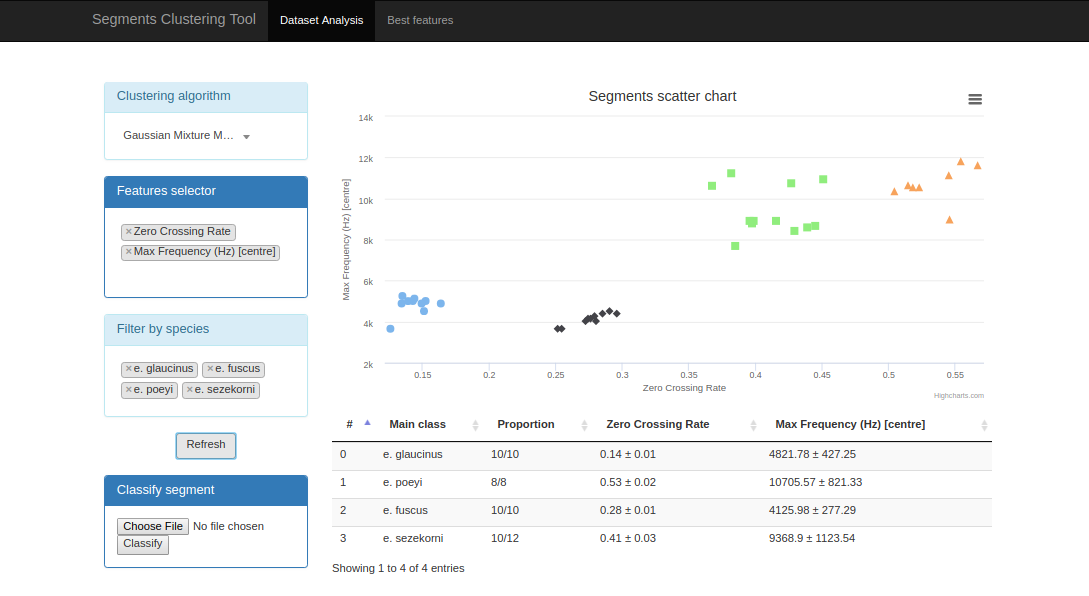
\includegraphics[width=\textwidth]{dataset-analysis.png}
    \caption{Vista de análisis de datos de la interfaz web de la herramienta \textit{Clusterapp}.}
    \label{img:dataset-analysis}
\end{figure}

\begin{figure}[!h]
    \centering
    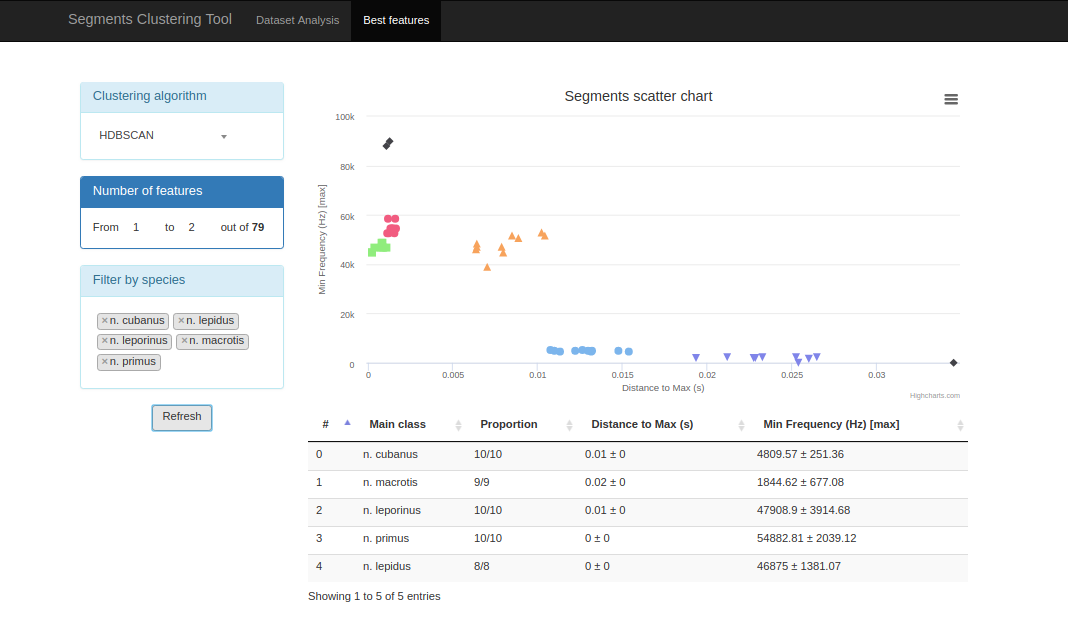
\includegraphics[width=\textwidth]{best-features.png}
    \caption{Vista de selección de las mejores características, de la interfaz web de la herramienta \textit{Clusterapp}.}
    \label{img:best-features}
\end{figure}

Las opciones de configuración en la interfaz web, así como la presentación de los resultados, varían en dependencia de si se dispone o no de información sobre la clasificación real de los segmentos de audio del conjunto de datos sobre el que se realiza el análisis.
Asimismo, en concordancia con dicha información se elige si será supervisado o no, el método para evaluar la calidad de los resultados de los algoritmos;
que es usado en la selección de las características que mejor diferencian los distintos tipos de vocalizaciones presentes en el conjunto de datos.

\subsection{Interfaz de línea de comandos}\label{subsec:CLI}

Mediante esta interfaz, usuarios de mayor experiencia empleando terminales de línea de comandos, pueden interactuar con la herramienta.
Si bien el número de configuraciones que ofrece esta variante es equivalente al de la interfaz web;
a diferencia de en aquella, las configuraciones no son introducidas de forma manual por el usuario, sino que se reciben en un fichero en formato \textit{JSON}.
Ello ofrece mayor rapidez en la ejecución de pruebas con variaciones en la configuración de la herramienta, y que dichas configuraciones puedan ser conservadas en disco para futuras réplicas de los resultados.

Adicionalmente la interfaz de línea de comandos ofrece una ventaja al presentar los resultados en forma más extensiva que su homóloga web.
Los valores obtenidos empleando las distintas medidas de evaluación son directamente mostrados en tablas.
Además, el usuario puede seleccionar si desea que los resultados del clustering con cada variación en la configuración se exporten a ficheros en formato \textit{JSON}, que pueden ser empleados por otras aplicaciones.

\subsection{Librería de Python}\label{subsec:libreríaDePython}

La librería de Python constituye la base sobre la que fueron implementadas las otras dos interfaces.
Se trata de una capa de abstracción entre el código que se encarga de la capa de presentación y el que realiza el cómputo científico.

Esta interfaz ofrece las mismas prestaciones que las ya mencionadas.
Su propósito radica en que puede ser empleada como base sobre la que implementar nuevas interfaces de interacción con el usuario, o para añadir las funcionalidades que provee la herramienta \textit{Clusterapp} directamente dentro de las interfaces de otras aplicaciones.

\section{Conjuntos de datos}\label{sec:datasets}

Para desarrollar los experimentos, se conformaron tres conjuntos de datos con segmentos correspondientes a vocalizaciones de dos \textit{clases} taxonómicas (aves e insectos) y un \textit{orden} taxonómico (murciélagos) respectivamente.
En las tablas~\ref{table:bats-dataset},~\ref{table:birds-dataset} y~\ref{table:insects-dataset} se describen las especies que componen cada uno de estos conjuntos.
Un cuarto conjunto de datos fue constituido a partir de la unión de los anteriores.
De esta forma se comprobó la variación en los resultados en dependencia del grado de parentesco existente entre las especies presentes en los conjuntos de datos.
Todos los segmentos se extrajeron de forma manual a partir de grabaciones de mayor duración.

La diversidad de sonidos que pueden producir los individuos de una misma especie, hace que en la clasificación de los segmentos no baste con recoger simplemente el nombre de la especie de la que proceden.
Por tal razón, se empleó además un identificador para distinguir entre tipos de vocalizaciones diferentes aun cuando estas pudieran provenir de individuos pertenecientes a la misma especie.
De esta forma es posible evaluar mejor los resultados de los algoritmos abordados en este trabajo;
pudiendo distinguirse así entre situaciones en que el algoritmo separó incorrectamente dos clusters de aquellas en que dicha acción tenía sentido por tratarse de tipos de vocalizaciones diferentes.

\section{Resultados}\label{sec:results}

Para la experimentación se emplearon todas las combinaciones de 14 de las características mencionadas en este trabajo:

\begin{multicols}{2}
    \begin{enumerate}
        \item \hyperref[subsec:log-attackTime]{Log-Attack Time}
        \item \hyperref[subsec:audioPower]{Audio Power}
        \item \hyperref[subsec:temporalCentroid]{Temporal Centroid}
        \item \hyperref[subsec:effectiveDuration]{Effective Duration}
        \item \hyperref[subsec:auto-correlation]{Auto-correlation}
        \item \hyperref[subsec:zeroCrossingRate]{Zero Crossing Rate}
        \item \hyperref[itemize:basic-spectral-features]{Frecuencia pico}
        \item \hyperref[itemize:basic-spectral-features]{Frecuencia máxima}
        \item \hyperref[itemize:basic-spectral-features]{Frecuencia mínima}
        \item \hyperref[itemize:basic-spectral-features]{Bandwidth}
        \item \hyperref[subsubsec:spectralCentroid]{Spectral Centroid}
        \item \hyperref[subsubsec:spectrallRollOff]{Spectral Roll-off}
        \item \hyperref[subsec:spectralFlux]{Spectral Flux}
        \item \hyperref[sec:MFCC]{MFCC}
    \end{enumerate}
\end{multicols}

En el caso de las características 2 y 5 se consideró la suma de todos los elementos de dichos vectores.
Para las numeradas entre 7 y 13, se consideró el promedio de los coeficientes correspondientes a las posiciones inicial, final, central, de valor máximo y de máxima amplitud del espectro.
Para los MFCC se empleó el vector obtenido al promediar cada uno de los coeficientes en el tiempo.

Los valores de algunas de las medidas de evaluación, aplicadas a los resultados obtenidos, aparecen resumidos en el Apéndice~\ref{ch:experimentsResults}.

En las figuras~\ref{img:bats},~\ref{img:birds},~\ref{img:insects} y~\ref{img:all} se resume la evaluación de los resultados aplicando el medidor \textit{Adjusted Rand Index};
para tres de estas combinaciones: la conformada por todas las características de la 1 a la 13 (nombradas características \textit{descriptivas}), la que solamente incluye los MFCC, y la que incluye a las 14 características.

\begin{figure}[!h]
    \centering
    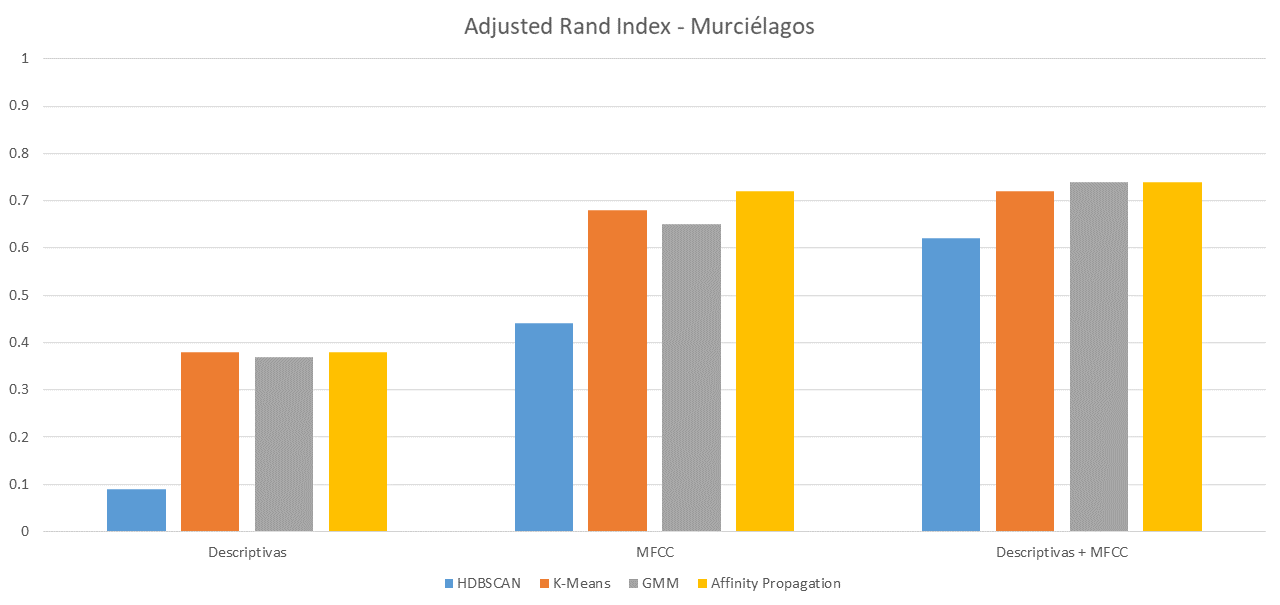
\includegraphics[width=\textwidth]{bats.png}
    \caption{Valores del criterio \textit{Adjusted Rand Index} para el conjunto de datos de murciélagos, en correspondencia con las características y el algoritmo de clustering empleado.}
    \label{img:bats}
\end{figure}

\begin{figure}[!h]
    \centering
    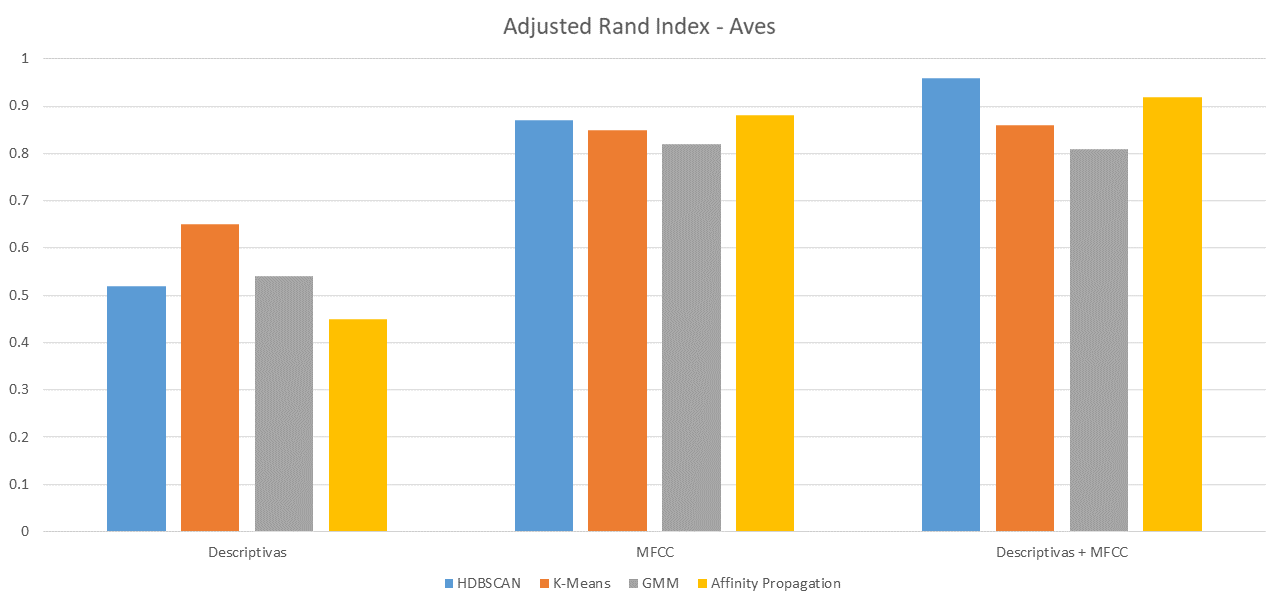
\includegraphics[width=\textwidth]{birds.png}
    \caption{Valores del criterio \textit{Adjusted Rand Index} para el conjunto de datos de aves, en correspondencia con las características y el algoritmo de clustering empleado.}
    \label{img:birds}
\end{figure}

\begin{figure}[!h]
    \centering
    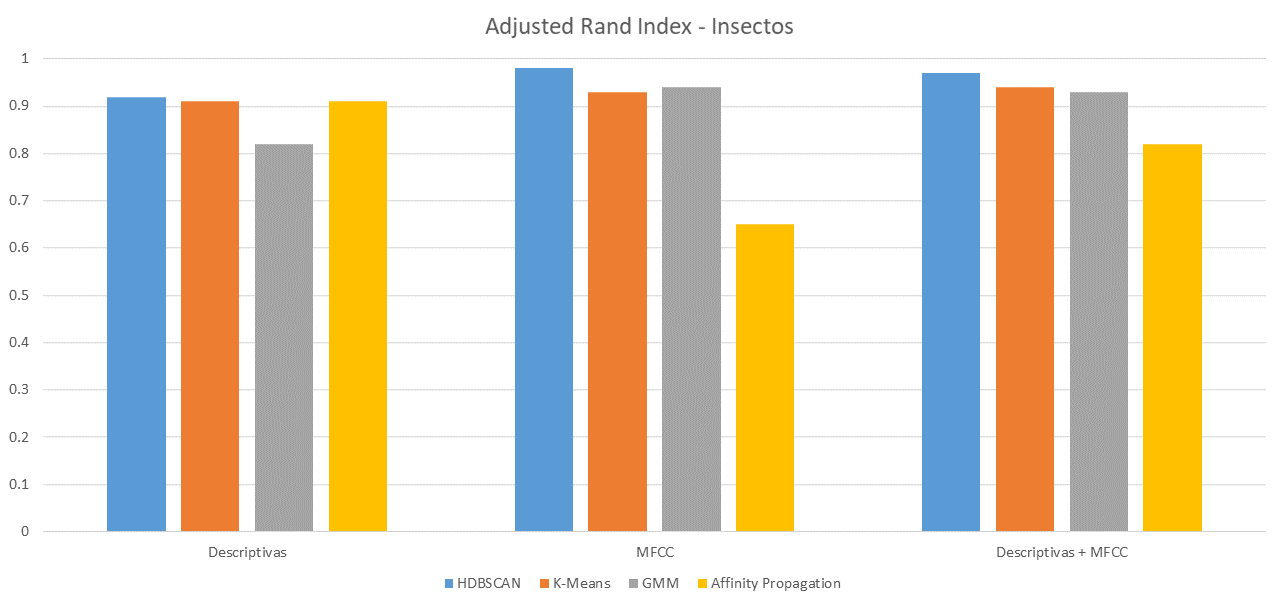
\includegraphics[width=\textwidth]{insects.png}
    \caption{Valores del criterio \textit{Adjusted Rand Index} para el conjunto de datos de insectos, en correspondencia con las características y el algoritmo de clustering empleado.}
    \label{img:insects}
\end{figure}

\begin{figure}[!h]
    \centering
    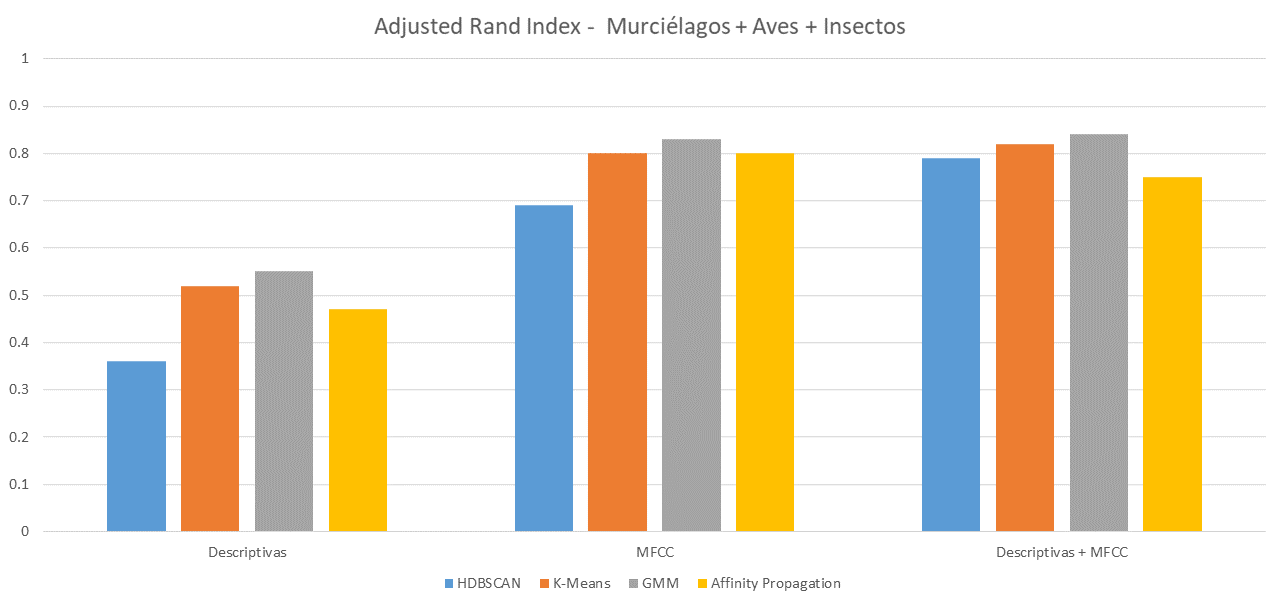
\includegraphics[width=\textwidth]{all.png}
    \caption{Valores del criterio \textit{Adjusted Rand Index} para el conjunto de datos conformado por la unión de los de murciélagos, aves e insectos, en correspondencia con las características y el algoritmo de clustering empleado.}
    \label{img:all}
\end{figure}

Se puede observar que en general los resultados son mucho mejores cuando los MFCC se encuentran presentes en las características utilizadas.
Si bien añadir características adicionales a dicho vector contribuye en la mayoría de los casos a incrementar la calidad del resultado, el valor en que lo hace no es muy significativo.

Puede apreciarse además que la selección del algoritmo no pesa tanto sobre la evaluación del resultado como lo hace la del conjunto de características.

En cuanto a la relación entre el parentesco taxonómico de las especies en el conjunto de datos y la evaluación de los resultados,
los obtenidos en este trabajo muestran mejor comportamiento cuando la diferencia entre las especies se da al nivel de \textit{clase}.
El resultado en el conjunto de los murciélagos soporta la hipótesis de que una relación más estrecha dentro del conjunto de datos deteriora un poco la calidad del resultado.
Lo mismo (aunque al parecer en menor grado) sucede en un conjunto de datos de alta diversidad de organismos.

\nomenclature{JSON}{JavaScript Object Notation}
\nomenclature{ARI}{Índice de Rand Ajustado (por sus siglas en inglés: Adjusted Rand Index)}
    %

    \backmatter

    %    \chapter*{Conclusiones}\label{ch:conclusion}
    %    En el presente trabajo se implementó un sistema para la aplicación de algoritmos de aprendizaje no supervisado en el estudio de señales bioacústicas.
Numerosas variantes de características de una señal de audio fueron incorporadas al sistema, así como algoritmos representativos de los diferentes modelos de clustering.

Los resultados obtenidos sobre cuatro conjuntos de datos, con diferentes grados de parentesco entre las especies, resultan alentadores;
y sugieren que el peso en el resultado final de los vectores de características con que se representen las señales, es mayor que el del algoritmo empleado.

La combinación de características que produce mejores resultados parece estar en estrecha correspondencia con cada conjunto de datos en particular.
No obstante, en la amplia mayoría de los casos se observó que los MFCC estuvieron presentes en las combinaciones con resultados de mayor calidad.
Asimismo, el uso de los MFCC como vector de características parece por sí solo dar muy buenos resultados, a los que la inclusión de características adicionales (altamente dependientes del conjunto de datos) parece mejorar solo hasta cierto punto.

\section*{Recomendaciones}\label{sec:recomendaciones}

Para dar continuidad al desarrollo de este trabajo, se recomienda verificar sus resultados en conjuntos de datos de mayor tamaño, que permitan dar validez estadística a los aquí planteados.

Este trabajo se enfocó en la generación de un resultado final de cara a su empleo directo por el usuario.
Es por ello que se propone como trabajo futuro comprobar su utilidad en pasos intermedios del proceso de estudio y clasificación de señales bioacústicas.
Un posible uso en este sentido pudiera ser la selección de los segmentos, donde en particular la habilidad de HDBSCAN de detectar datos de <<ruido>> puede tener buen empleo.

Otro posible uso como paso intermedio puede darse en la mejora de la clasificación de los elementos de un conjunto de datos.
De esta forma si se dispone solamente de la especie que emitió cada uno de los segmentos, el cluster en que estos se ubiquen puede ser considerado un indicador del tipo de vocalización.
Así, si los segmentos correspondientes a la misma especie aparecen repartidos en dos clusters, esto señalaría que existen dos tipos de vocalizaciones diferentes;
información que pudiera añadirse a la clasificación de los segmentos.


    \selectbiblanguage{spanish}
    \bibliographystyle{babplain-lf}
    \bibliography{references}

    %    \appendix
    %    \chapter{Appendix Title}\label{ch:appendix}
    %    \input{chapters/appendix}

\end{document}